%% ****** Start of file aiptemplate.tex ****** %
%%
%%   This file is part of the files in the distribution of AIP substyles for REVTeX4.
%%   Version 4.1 of 9 October 2009.
%%
%
% This is a template for producing documents for use with 
% the REVTEX 4.1 document class and the AIP substyles.
% 
% Copy this file to another name and then work on that file.
% That way, you always have this original template file to use.

%\documentclass[aip,graphicx]{revtex4-1}
%\documentclass[aip,reprint]{revtex4-1}

%\usepackage{graphicx}

%\draft % marks overfull lines with a black rule on the right
%\documentclass[pre,aps,floatfix,authordate1-4,twocolumn]{revtex4-1}
%\documentclass[pre,aps,floatfix,authordate1-4]{revtex4-1}

\documentclass[aps,prl,superscriptaddress,twocolumn]{revtex4}



%\documentclass[aps,prl,preprint,groupedaddress]{revtex4}

\usepackage{rotating} 
\usepackage{times}
\usepackage{graphicx}
\usepackage{setspace}
\usepackage{amsmath}
\usepackage{epstopdf}
\usepackage[obeyFinal]{easy-todo}
\usepackage{csquotes}
\usepackage{xr}
\externaldocument{manuscriptPGPEsuppl}


\begin{document}

% Use the \preprint command to place your local institutional report number 
% on the title page in preprint mode.
% Multiple \preprint commands are allowed.
%\preprint{}

\title{NMRlipids IV: Headgroup \& glycerol backbone structures, and cation binding in bilayers with PE and PG lipids} %Title of paper

% repeat the \author .. \affiliation  etc. as needed
% \email, \thanks, \homepage, \altaffiliation all apply to the current author.
% Explanatory text should go in the []'s, 
% actual e-mail address or url should go in the {}'s for \email and \homepage.
% Please use the appropriate macro for the type of information

% \affiliation command applies to all authors since the last \affiliation command. 
% The \affiliation command should follow the other information.

\author{Am{\'e}lie Bacle}
\affiliation{Paris, France}

\author{Pavel Buslaev}
\affiliation{University of Jyv{\"a}skyl{\"a}}

\author{Rebeca Garc{\'i}a Fandi{\~n}o}
\affiliation{Center for Research in Biological Chemistry and Molecular Materials (CiQUS), Universidade de Santiago de Compostela, E-15782 Santiago de Compostela, Spain}
\affiliation{CIQUP, Centro de Investigação em Química, Departamento de Química e Bioquímica, Faculdade de Ciências, Universidade do Porto, Porto, Portugal}

\author{Fernando Favela-Rosales}
\affiliation{Departamento de Investigaci\'{o}n, Tecnol\'{o}gico Nacional de M\'{e}xico, Campus Zacatecas Occidente, M\'{e}xico}

\author{Patrick Fuchs}
\affiliation{Paris, France}

\author{Matti Javanainen}
\affiliation{Institute of Organic Chemistry and Biochemistry of the 
Czech Academy of Sciences, Flemingovo n\'{a}m. 542/2, CZ-16610 Prague 6, Czech Republic}

\author{Jesper J. Madsen}
\affiliation{Department of Chemistry, The University of Chicago, Chicago, Illinois, United States of America}
\affiliation{Department of Global Health, College of Public Health, University of South Florida, Tampa, Florida, United States of America}

\author{Josef Melcr}
\affiliation{Institute of Organic Chemistry and Biochemistry of the 
Czech Academy of Sciences, Flemingovo n\'{a}m. 542/2, CZ-16610 Prague 6, Czech Republic}
\affiliation{Groningen Biomolecular Sciences and Biotechnology Institute 
and The Zernike Institute for Advanced Materials, 
University of Groningen, 9747 AG Groningen, The Netherlands}

\author{Paula Milan Rodriguez}
\affiliation{Paris, France}

\author{Markus S. Miettinen}
% \affiliation[Max Planck Institute of Colloids and Interfaces]{Department of Theory and Bio-Systems, Max Planck Institute of Colloids and Interfaces, 14424 Potsdam, Germany}
\affiliation{Department of Theory and Bio-Systems, Max Planck Institute of Colloids and Interfaces, 14424 Potsdam, Germany}

\author{O. H. Samuli Ollila}
\email[]{samuli.ollila@helsinki.fi}
\affiliation{Institute of Biotechnology, University of Helsinki}

\author{Chris G. Papadopoulos}
\affiliation{I2BC - University Paris Sud}


\author{Antonio Pe{\'o}n}
\affiliation{Spain}

\author{Thomas J. Piggot}
\affiliation{Chemistry, University of Southampton, Highfield, Southampton SO17 1BJ, United Kingdom}

\author{{\'A}ngel Pi{\~n}eiro}
\affiliation{Departamento de F{\'i}sica Aplicada, Facultade de F{\'i}sica, Universidade de Santiago de Compostela, E-15782 Santiago de Compostela, Spain}

\author{Pierre Poulain}
\affiliation{Paris, France}

% Collaboration name, if desired (requires use of superscriptaddress option in \documentclass). 
% \noaffiliation is required (may also be used with the \author command).
%\collaboration{}
%\noaffiliation

\date{\today}

\begin{abstract}
% insert abstract here
  Chemistry of lipid headgroups, the water facing components of cell membranes, varies between organisms and
  organelles and regulate cell functions via lipid-protein interactions.
  Because lipid membranes are in liquid state in physiological conditions,
  the conformational ensembles of lipids and their dependence of headgroup chemistry are difficult to resolve experimentally.
  Here, we combine solid state NMR experiments and MD simulations from NMRlipids open collaboration to
  resolve conformational ensembles of PC, PS, PG and PE lipid headgroups in liquid lamellar phase in various biologically relevant conditions.
  Interpretation of NMR experiments using the best simulations from the NMRlipids project suggests that all lipid headgroups sample wide range of
  conformations in neutral and charged cell membranes, and that the differences in headgroup chemistry
  appears in the probability weights of different conformations. Together with the analysis of protein-bound-lipids
  from the protein data bank (PDB), this suggests that lipids can bind to proteins in wide range of conformations
  independently on the headgroup chemistry. Therefore, the specific lipid-protein interactions are likely driven by
  protein-lipid interactions, rather than conformational restrictions of lipids. Our results paves the way to
  comprehensive understanding of lipid-protein interaction energetics, and understanding complex biomolecular assemblies
  such as membrane proteins.

  %The force field giving the best description for glycerol backbone and headgroup structures
  %of PC, PS, PG and PE headgroups (CHARMM36) reproduces the essential differences in order parameters
  %between these headgroups, and therefore enables the analysis of structural differences between the
  %headgroups.


\end{abstract}

%\pacs{}% insert suggested PACS numbers in braces on next line

\maketitle %\maketitle must follow title, authors, abstract and \pacs

% Body of paper goes here. Use proper sectioning commands. 
% References should be done using the \cite, \ref, and \label commands


%\label{}
\section{Introduction}

Chemical compositions of hydrophilic lipid headgroups vary between different
organelles and organisms, and different lipid types
regulate protein functions in many different ways \cite{lee03,vanmeer08}.
Lipids can directly bind to proteins or indirectly affect protein
functions by altering membrane properties or charge \cite{lee03,lemmon08}.
While the specific interactions with certain lipid headgroups
are known to be essential for the function of several proteins \cite{lee11,lemmon08},
it is not clear if the specificity is driven by the differences in accessible
conformational states between lipid types or
by specific intermolecular lipid-protein interactions.

Lipid conformational ensembles in physiologically relevant lamellar liquid phase
are typically derived from NMR experiments, particularly from 
%Attempts to resolve the conformational ensembles of lipid headgroup rely mainly on
C-H bond order parameters measured using $^2$H NMR~\cite{seelig77c,davis83,Semchyschyn04}
which can be detected even from cells \cite{gally81,scherer87,seelig90}.
%but lipids are not in solid state in biomembranes. 
%On the other hand, NMR experiments enable detection of lipid headgroups
%in physiological liquid states also in cells \cite{gally81,scherer87,seelig90}.
These studies suggest that the glycerol backbone structures are largely similar irrespectively of the headgroup \cite{gally81}, 
and the headgroup structures are similar in PC, PE and PG lipids, while headgroup is more rigid in PS lipids \cite{wohlgemuth80,buldt81}. 
%Extensive discussion about structural details of PE, PG or PS headgroups do not exists (as far as I know), 
%In contrast to PC lipids (see \cite{botan15} and references therein).
%Some attempts to resolve conformational ensembles from NMR for PC and PE lipids have been made,
%but lesser extend for PG or PS lipids \cite{seelig77c,davis83,Semchyschyn04}.
However, these results are based only on the absolute values while 
%we have recently demonstrated that also
the necessity of order parameters signs in capturing the lipid conformational ensembles has been resently demonstrated \cite{botan15,ollila16,ferreira16}.
Furthermore, the detailed understanding of lipid conformational ensembles
is limited by the lack of universal models to interpret the experiments \cite{pezeshkian18,akutsu20}.
%do not exist and
%the proposed structures are often based on lipid crystal structures \cite{pezeshkian18,akutsu20}.
%which were solved many decades ago \cite{buldt81,pascher92}.
%determine the structural 
%Classical molecular dynamics simulations could potentially give such ensembles and therefore enable
%the detailed studies of lipid headgroup behaviour in complex biomolecular systems, but current
%force fields are not accurate enough to reproduce the correct conformational ensembles for PC and PS headgroups \cite{botan15,antila19}.

Stuctures of different lipid types in protein bound states can be extracted from the protein data bank (PDB) \cite{berman00},
but their relation to the conformational ensembles in liquid lamellar state remains unclear \cite{marsh13b}.
In addition to the changes in lipid conformational ensembles upon binding to proteins,
%PC headgroup conformations do not change upon addition of zwitterionic lipids or cholesterol \cite{scherer87,ferreira13} into a membrane,
%but are sensitive to the presence of charged molecules in membranes \cite{seelig87}.
also the experimentally measured response of lipid headgroup to membrane bound charges remains poorly understood 
%The response to charges is explained by the change in the orientation of lipid headgroup dipole vector due to electrostatic interactions,
%but the detailed changes are not yet understood
due to the lack of suitable models to interpret the lipid conformational ensembles in liquid lamellar state \cite{Semchyschyn04}.


Here, we use natural abundance $^{13}$C NMR experiments and MD simulations from the NMRlipids open collaboration
to resolve the differences in conformational ensembles between PC, PE, PG and PS lipid headgroups.
%open collaboration and order parameters of glycerol backbone and headgroup
%to evaluate the accuracy of PE and PG heagroup structures, and the cation binding affinity
Zwitterionic PC and PE are the most common lipids in eukaryotes and bacteria, respectively \cite{vanmeer08,sohlenkamp16}.
PE is also the second most abundant glycerophospholipid in eukaryotic cells
and has been related to various diseases \cite{vance15,calzada16,patel17}.
PS and PG are the most common negatively charged lipids in eukaryotes and bacteria, respectively,
and affect membrane protein functionality and signaling \cite{lemmon08,leventis10,sohlenkamp16,hariharan18}.
%PE and PG lipids are most common lipids in bacteria \cite{sohlenkamp16}.
%Anionic PG lipids are less abundant, but is also proposed to be fundamental for terrestrial life \cite{furse17}.
%PE and PG affect membrane protein functionality \cite{hariharan18} and
All the studied lipids specifically bind to various proteins \cite{yeagle14}.
%PE headgroup is also prone for negative membrane curvature and causes membrane fusion \cite{Chernomordik08,calzada16}.
%Therefore, the PE and PG headgroup structures play probably essential roles in 
%many biological processes.
Furthermore, we use our results to elucidate lipid-protein interactions and the effect of charges on lipid conformations.

The lipid conformational ensembles in liquid lamellar state paves the way toward understanding the
specific binding of different lipid types to membrane proteins and how they regulate the protein function.
Because glycerol backbone and headgroup structures of PC lipids are similar in model membranes and in bacteria \cite{gally81,scherer87,seelig90},
the results from model systems could be used to understand the biological role of lipid headgroup conformational ensembles in different lipid types.

%Several MD simulations of PE and PG lipids have been published especially in the context of modeling
%inner membrane of Gram-negative
%bacteria \cite{devries04,murzyn05,pedersen06,zhao07,gurtovenko08,zhao08,henin09,kukol09,tsai12,dickson12,venable13,dickson14,berglund15}
%\todo{There may be some relevant publication missing from here},
%but evaluation of glycerol backbone and headgroup structures against experiments is rare \cite{henin09}.

%Derivation of different lipid headgroup conformational ensembles in liquid state has been
%inconclusive due to lack of suitable experimental data and tools to interpret the conformational ensembles.


%Besides the structure, also ion binding may regulate biophysical activity of especially negatively
%charged lipid headgroups \cite{seelig90}. Monovalent cation (except Lithium) binding to zwitterionic PC and anionic PS headgroups is
%very weak, while multivalent ion binding is stronger but still weak \cite{cevc90,tocanne90,roux90,catte16,antila19}. The ion binding affinity
%data for PE is more scarce \cite{marra85}, but large differences to PC would be surprising.
%Negatively charged lipids are suggested to bear same cation binding constants than zwitterionic lipids, but
%the amount of bound ions to negatively charged membranes would still be larger because
%the concentration of cations in the vicinity of membranes would be higher  \cite{seelig90}.
%
%is stronger
%Based on the electrometer concept and other data is has been suggested that \cite{seelig90}
%\begin{displayquote}
%  {\it ''(i) Ca$^{2+}$ binds to neutral lipids (phosphatidylcholine, phosphatidylethanolamine) and negatively charged lipids
%    (phosphatidylglycerol) with approximately the same binding constant of K = 10-20 M$^{-1}$; \\
%    (ii) the free Ca$^{2+}$
%    concentration at the membrane interface is distinctly enhanced if the membrane carries a negative surface
%    charge, either due to protein or to lipid; \\
%    (iii) increased inter-facial Ca$^{2+}$ also means increased amounts
%    of bound Ca$^{2+}$ at neutral and charged lipids; \\
%    (iv) the actual binding step can be described by a Langmuir
%    adsorption isotherm with a 1 lipid:1 Ca$^{2+}$ stoichiometry, provided the interfacial concentration C$_M$, is
%    used to describe the chemical binding equilibrium.''}
%\end{displayquote}
%
%On the other hand, anionic PS lipids are proposed chelate with calcium ions \cite{hauser85,feigenson86,roux91}.
%In simulations, the cation binding affinity to PC and PS membranes is typically overestimated \cite{catte16,antila19},
%which can be improved by applying the ECC to the partial charges of the force fields \cite{melcr18,melcr19}.


%\begin{figure}[]
%  \centering
%  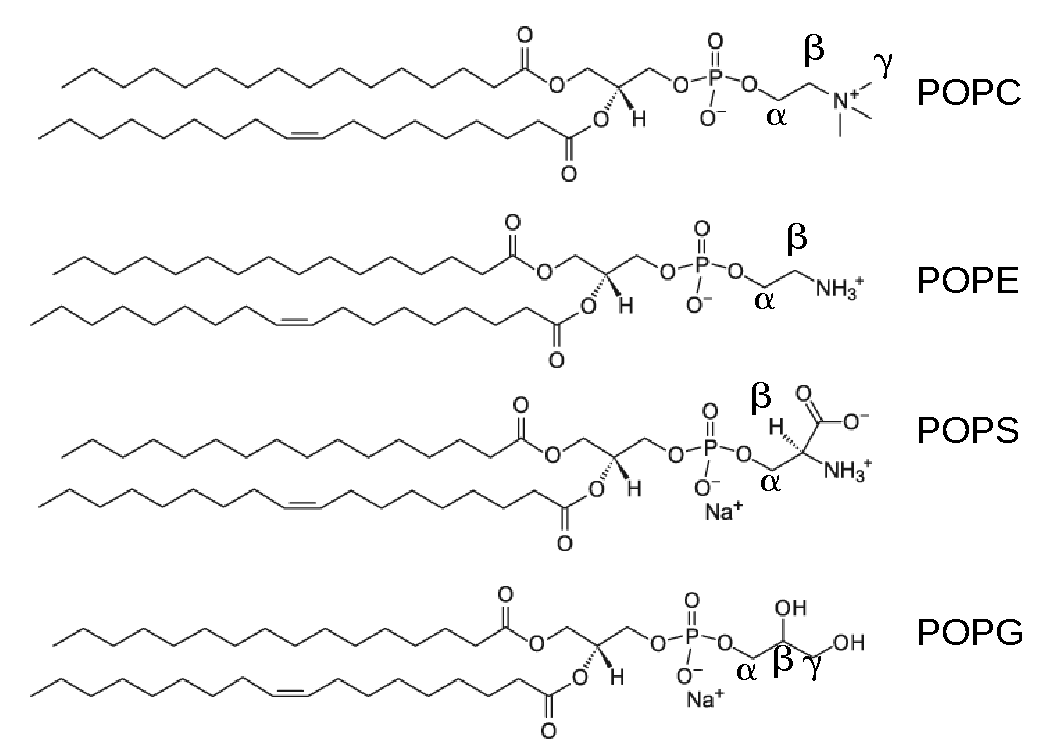
\includegraphics[width=9.0cm]{../Figs/lipids.pdf}
%  \caption{\label{lipids}
%    Chemical structures and labels for the headgroup carbons.
%  }
%\end{figure}



\section{Methods}
\subsection{Experimental C--H bond order parameters}
The headgroup and glycerol backbone C--H bond order parameters of POPE and POPG
were measured using natural abundance $^{13}$C solid state NMR spectroscopy
as described previously \cite{ferreira13,ferreira16}.
The magnitudes of order parameters were determined from the chemical-shift resolved dipolar splittings
using a R-type Proton Detected Local Field (R-PDLF) experiment~\cite{dvinskikh04} and
the signs from S-DROSS experiments~\cite{gross97} combined with SIMPSON simulations \cite{bak00}.
%The experiments were done in a Bruker Avance III 400 spectrometer operating at a $^1$H Larmor frequency of 400.03 MHz.
%Magic angle spinning (MAS) of the sample was used at a frequency of 5.15 kHz (R-PDLF experiment) and 5 kHz (S-DROSS experiment).
%The following experimental setups were used.
The NMR experiments were identical as in our previous work~\cite{antila19}.
POPE and POPG powder were purchased from Avanti polar lipids \todo{Which isomer of POPG we have in the experiments?}.
%\todo{Is this enough and correct, or should we repeat some methods from the NMRlipidsIVps paper?}
The POPE experiments were recorded at 310~K and POPG experiments at 298~K, where the bilayers are in the liquid disordered phase \cite{marsh13}.

%Absolute values of the headgroup and glycerol backbone order parameters from PE and PG lipids are measured
%previously using $^2$H NMR~\cite{seelig76,gally81,wohlgemuth80,borle85}. Because also the order parameter
%signs bear essential information about the lipid structures \cite{botan15,ollila16}, we measured the
%magnitudes and signs of POPE and POPG C--H bond headgroup and glycerol backbone order parameter in liquid phase
%using the 2D-RPDLF and S-DROSS experiments, as described previously \cite{ferreira13,ferreira16,antila19}.

Glycerol backbone peaks from both lipids, and $\alpha$-carbon peak from POPE in the INEPT spectra 
were assigned based on previously measured POPC spectra~\cite{ferreira13}.
%For POPE, the glycerol backbone and $\alpha$-carbon peaks in INEPT spectra were assigned based on
%previously measured POPC spectra~\cite{ferreira13} and
The $\beta$-carbon peak from POPE was assigned based on $^{13}$C chemical shift table for amines available
at \url{https://www.chem.wisc.edu/areas/reich/nmr/c13-data/cdata.htm}.
%For POPG, the glycerol backbone peaks in INEPT spectra were assigned based on
%previously measured POPC spectra~\cite{ferreira13},
\todo{How were $\alpha$ and  $\gamma$-carbon peaks assigned in POPG?}.
The $\beta$-carbon peak from POPG overlapped with the g$_2$ peak from glycerol backbone
because their chemical environments are similar in POPG.
\todo{Details to be checked by Tiago}.

\subsection{Molecular dynamics simulations}

Molecular dynamics simulation data were collected using
the NMRlipids Open Collaboration \cite{botan15}, which is running at
\url{nmrlipids.blogspot.fi} and \url{github.com/NMRlipids/NMRlipidsIVotherHGs}.
The simulated systems of pure PE and PG bilayers without additional ions
are listed in Tables \ref{systemsPE} and \ref{systemsPG},
and lipid mixtures with additional ions in Table~\ref{systemsMIX}.
Further simulation details are given in the SI, and
the simulation data are indexed in a
searchable database available at \url{www.nmrlipids.fi},
and in the NMRlipids/MATCH repository (\url{github.com/NMRlipids/MATCH}).

\subsection{Analysis of molecular dynamics simulation data}
The big data set of MD simulations was analysed in the NMRlipids databank manner.
Unique naming convention for lipid atoms in each force field was defined using the mapping files
and analysis for all simulations indexed in NMRlipids databank manner were performed
using python codes.

The C--H bond order parameters were calculated directly
from the carbon and hydrogen positions using the definition
\begin{equation}
S_{\rm CH}=\frac{1}{2}\langle 3\cos^2\theta -1 \rangle,
\end{equation}
where $\theta$ is the angle between the C--H bond and the membrane normal
(taken to align with $z$, with bilayer periodicity in the $xy$-plane).
Angular brackets denote average over all sampled configurations.
The order parameters were first calculated averaging over time separately
for each lipid in the system. The average and
the standard error of the mean were then calculated over different lipids.
Python programs that use the MDAnalysis library \cite{agrawal11,gowers16}
used for all atom simulations is available in Ref. \citenum{MATCHgit}
({\tt scripts/calcOrderParameters.py}). For united atom simulations, the trajectories
with hydrogens having ideal geometry were constructed first using either buildH program~\cite{buildH}
or ({\tt scratch/opAAUA\_prod.py}) in  Ref. \citenum{MATCHgit}, and the order parameters were
then calculated from these trajectories. This approach has been tested against trajectories
with explicit hydrogens and the deviations in order parameters are small \cite{buildH,piggot17}.\\
\todo{BuildH program is now cited with a direct link to the GitHub repo. I think that a release to Zenodo would be nice in the final publication.}\\
\todo{Maybe we should also shortly discuss here about the reasons for slight dependence of order parameter values on the method used to reconstruct hydrogens?}\\
The ion number density profiles were calculated using the {\tt gmx density} tool
of the Gromacs sofware package \cite{gromacsMANUAL}.

%\clearpage
\begin{figure*}[]
  \centering
%  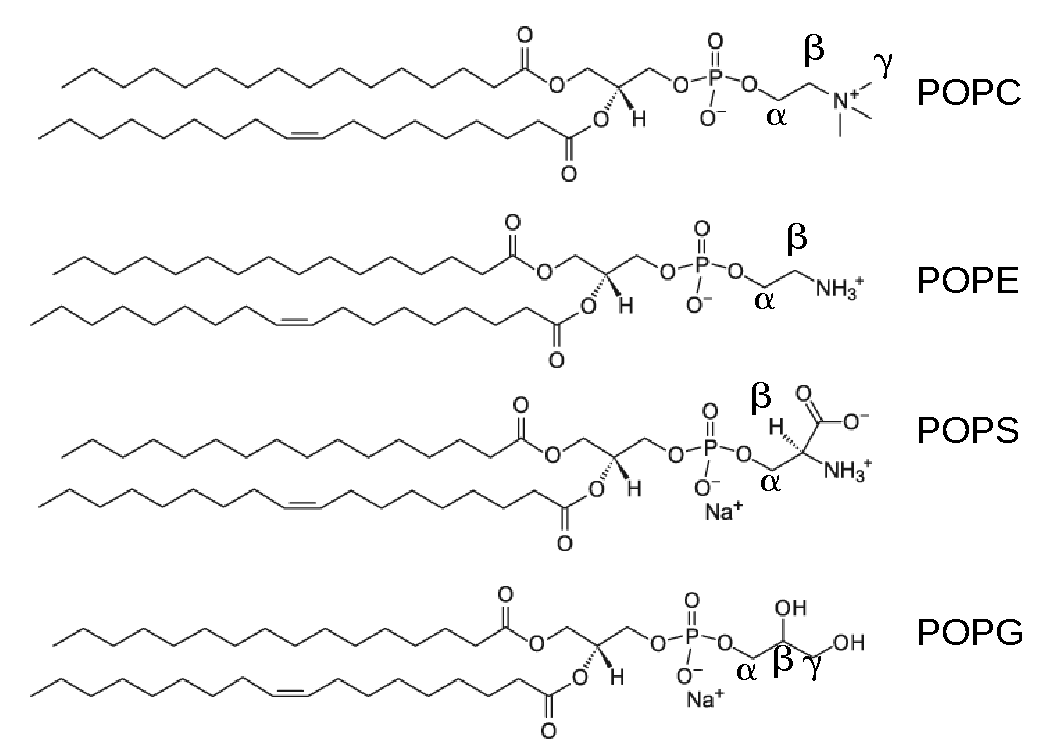
\includegraphics[width=9.0cm]{../Figs/lipids.pdf}
  %  \includegraphics[width=9.0cm]{../Figs/HGorderparametersPCPSPEPG.eps}
   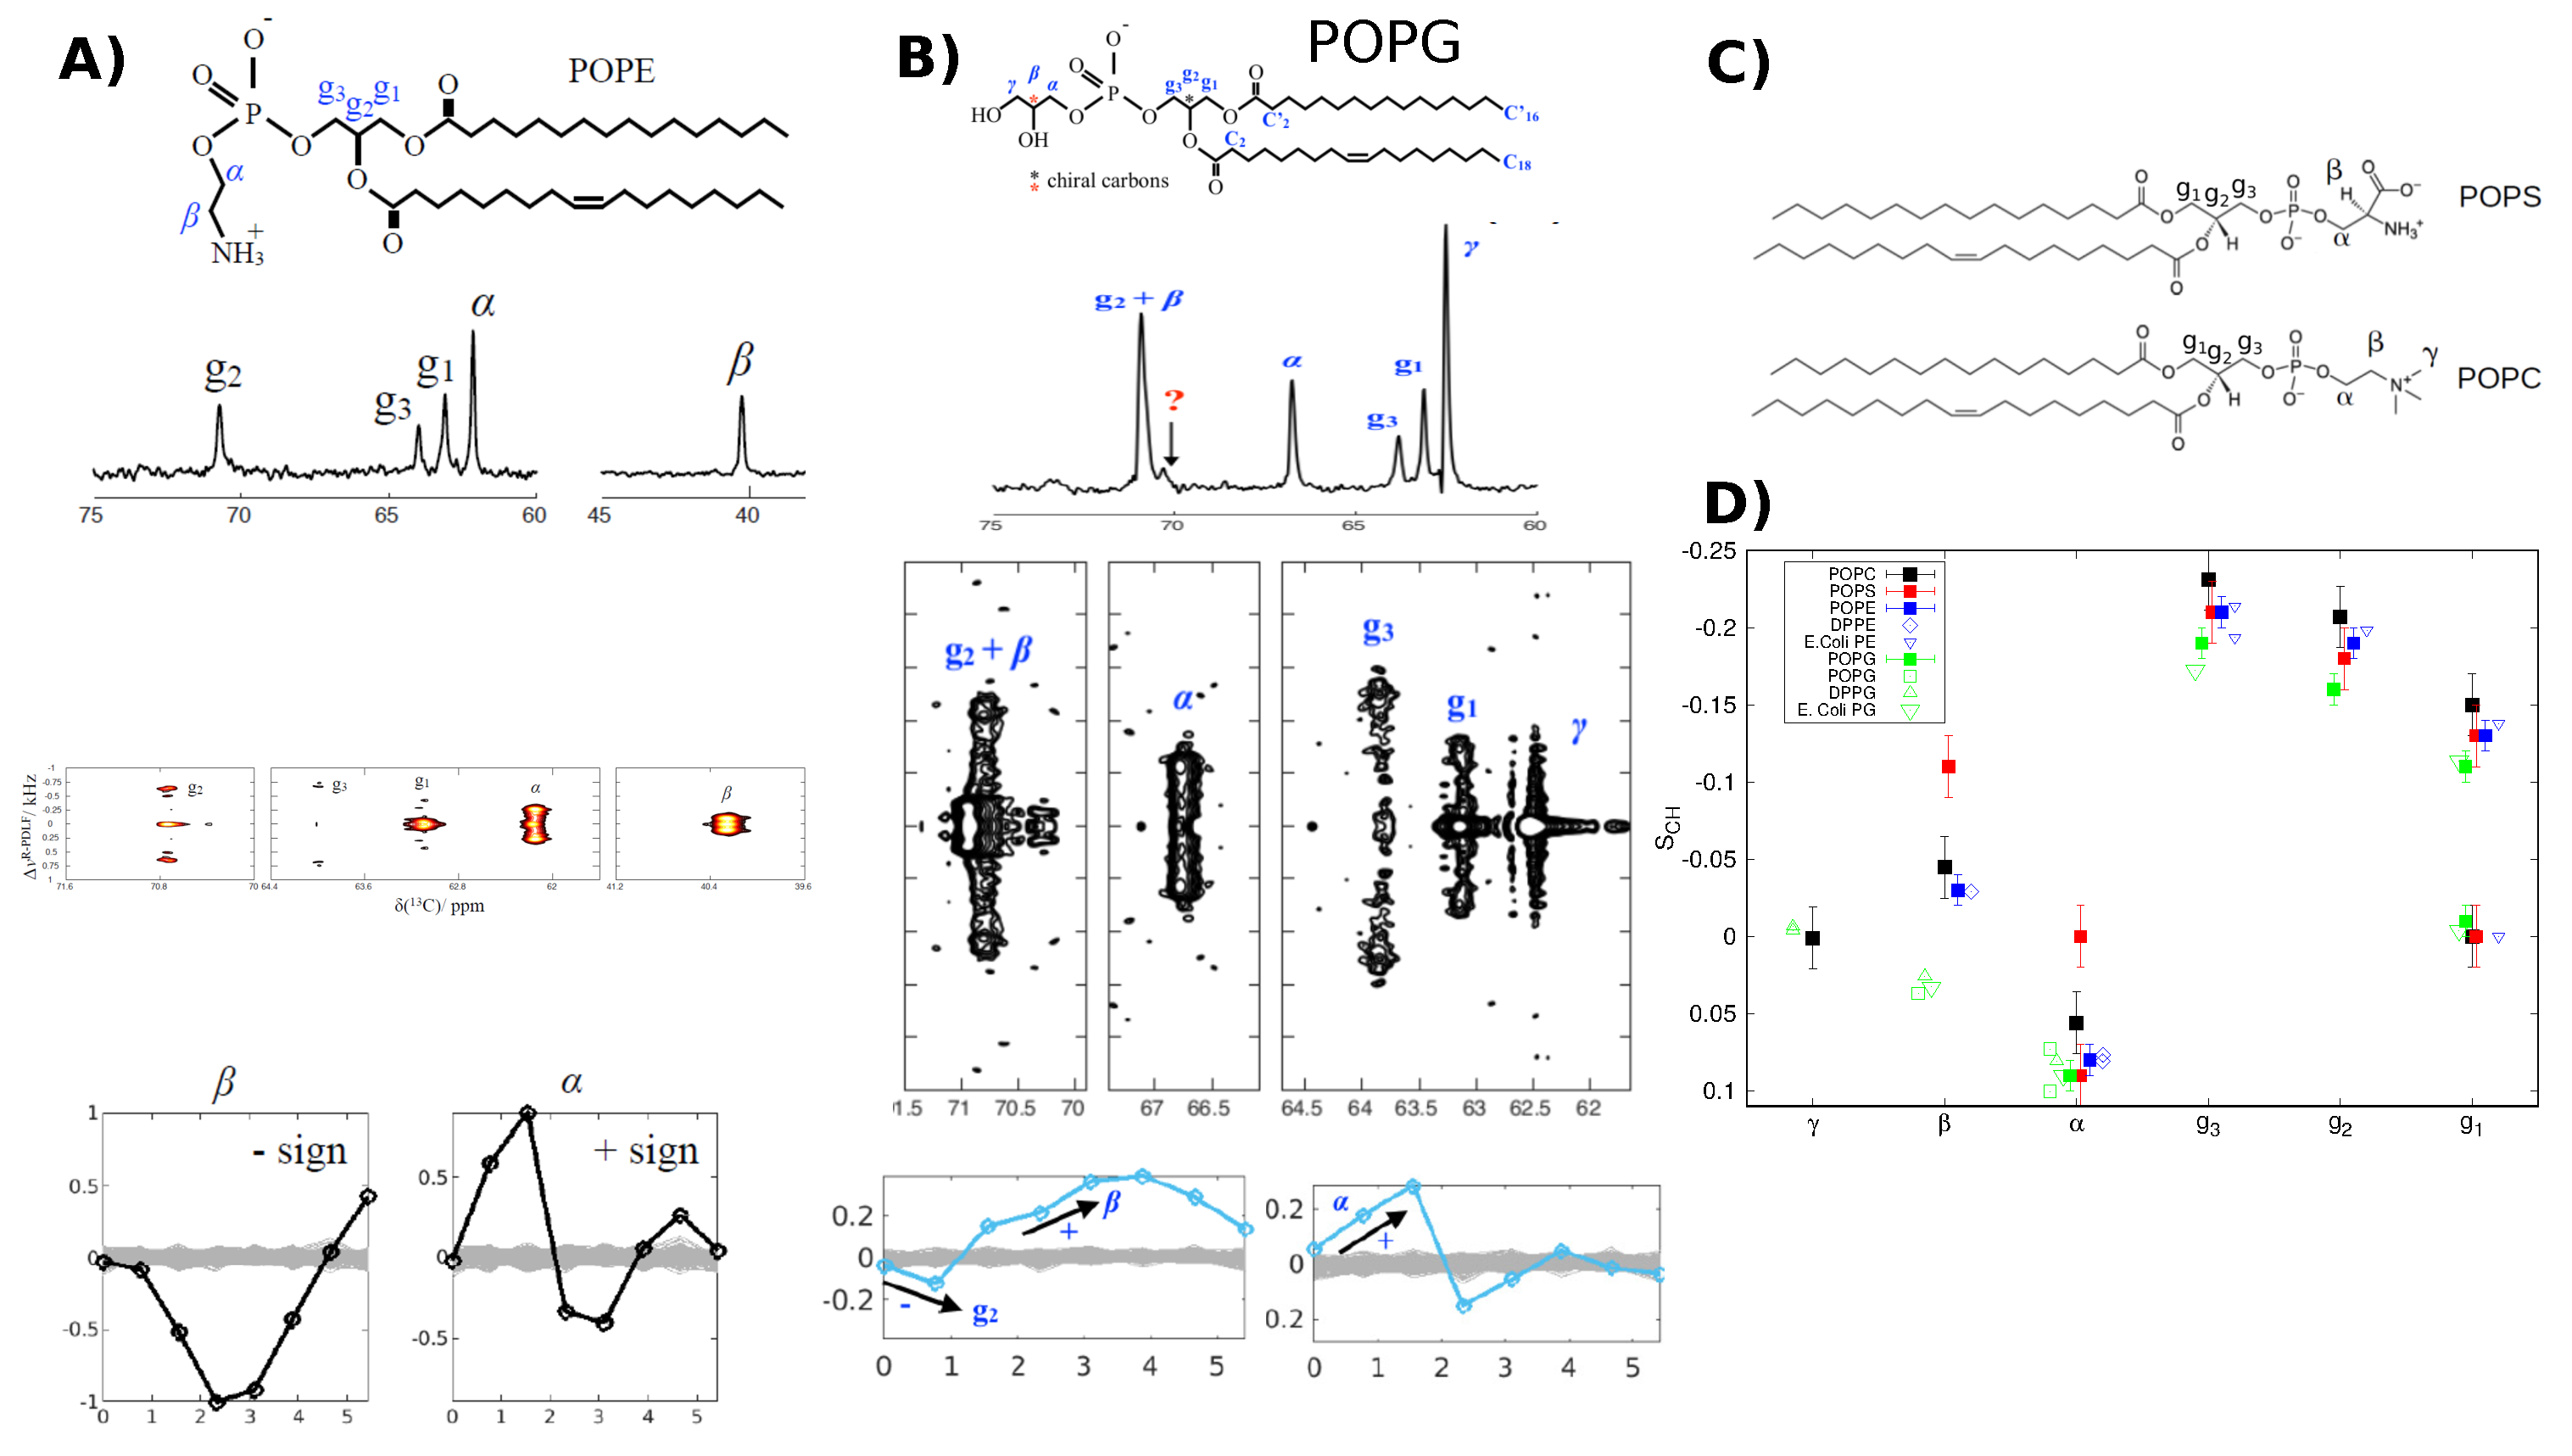
\includegraphics[width=18.0cm]{../Figs/figure1.eps}
   \caption{\label{HGorderParameters}
     Chemical structure, refocused-INEPT spectrum, 2D R-PDLF spectra, and S-DROSS data (from top to bottom) of {\bf A)} POPE  and {\bf B)} POPG.
      Full NMR spectra are shown Figs. \ref{POPEspectra} and \ref{POPGspectra}.
     {\bf C)} Chemical structure of POPC and POPS.
    {\bf D)} Headgroup and glycerol backbone order parameters from different experiments in lamellar liquid disordered phase.
    The values and signs for POPE (310~K) and POPG (298~K)
    measured in this work, and for POPS (298~K) \cite{antila19} and POPC (300~K) \cite{ferreira13,ferreira16}
    previously using $^{13}$C NMR. The literature values for
    DOPS with 0.1M of NaCl (303~K) \cite{browning80},
    POPG with 10nM PIPES (298~K) \cite{borle85},
    DPPG with 10mM PIPES and 100mM NaCl (314~K) \cite{wohlgemuth80}, 
    DPPE (341~K) \cite{seelig76},
    E.coliPE and E.coliPG (310~K) \cite{gally81}
    are measured using $^2$H NMR. The signs from $^{13}$C NMR are used also for the literature values.
   }
   \todo{This is a sketch, Tiago Ferreira will make a new figure.} \\
%  \todo{D) could be clarified as Fig. 2 in the NMRlipids IVps paper.}
\end{figure*}


\subsection{Analysis of lipid conformations bound to proteins}
Lipid structures from PDB (\url{http://www.rcsb.org/})
were searched using PDBe REST API (\url{www.ebi.ac.uk/pdbe/pdbe-rest-api}).
First, all PDB entries containing PC, PE, PG, or PS lipid headgroups were searched.
The ligand names to identify the lipids were:
PLC, PX4, 6PL, LIO, HGX, PC7, PC8, P1O, 6O8, XP5, EGY, PLD, SBM, HXG, and PCW for PC;
8PE, PTY, 3PE, PEH, PEF, 6OE, 6O9, 9PE, PEV, 46E, SBJ, L9Q, PEK, EPH, ZPE, 9TL, 9Y0, 6OU, LOP, and PEE for PE;
PGT, PGK, LHG, 44G, PGV, OZ2, D3D, PGW, DR9, P6L, PG8, H3T, and GOT for PG; and
PSF, PS6, Q3G, P5S, D39, PS2, 17F, and 8SP for PS.
All PDB structures containing these ligands were downloaded and the dihedral angles of
the first lipid in the latest version of the structures within each PDB code were calculated  
using MDTraj python library \cite{mcgibbon15}.
The used Jupyter notebook is available from the project's GitHub repository ({\it scripts/pdbSEARCH.ipynb}).



\section{Results and Discussion}

%\subsection{Headgroup and glycerol backbone order parameters of POPE and POPG from $^{13}$C NMR}

\begin{figure*}[]
  \centering
   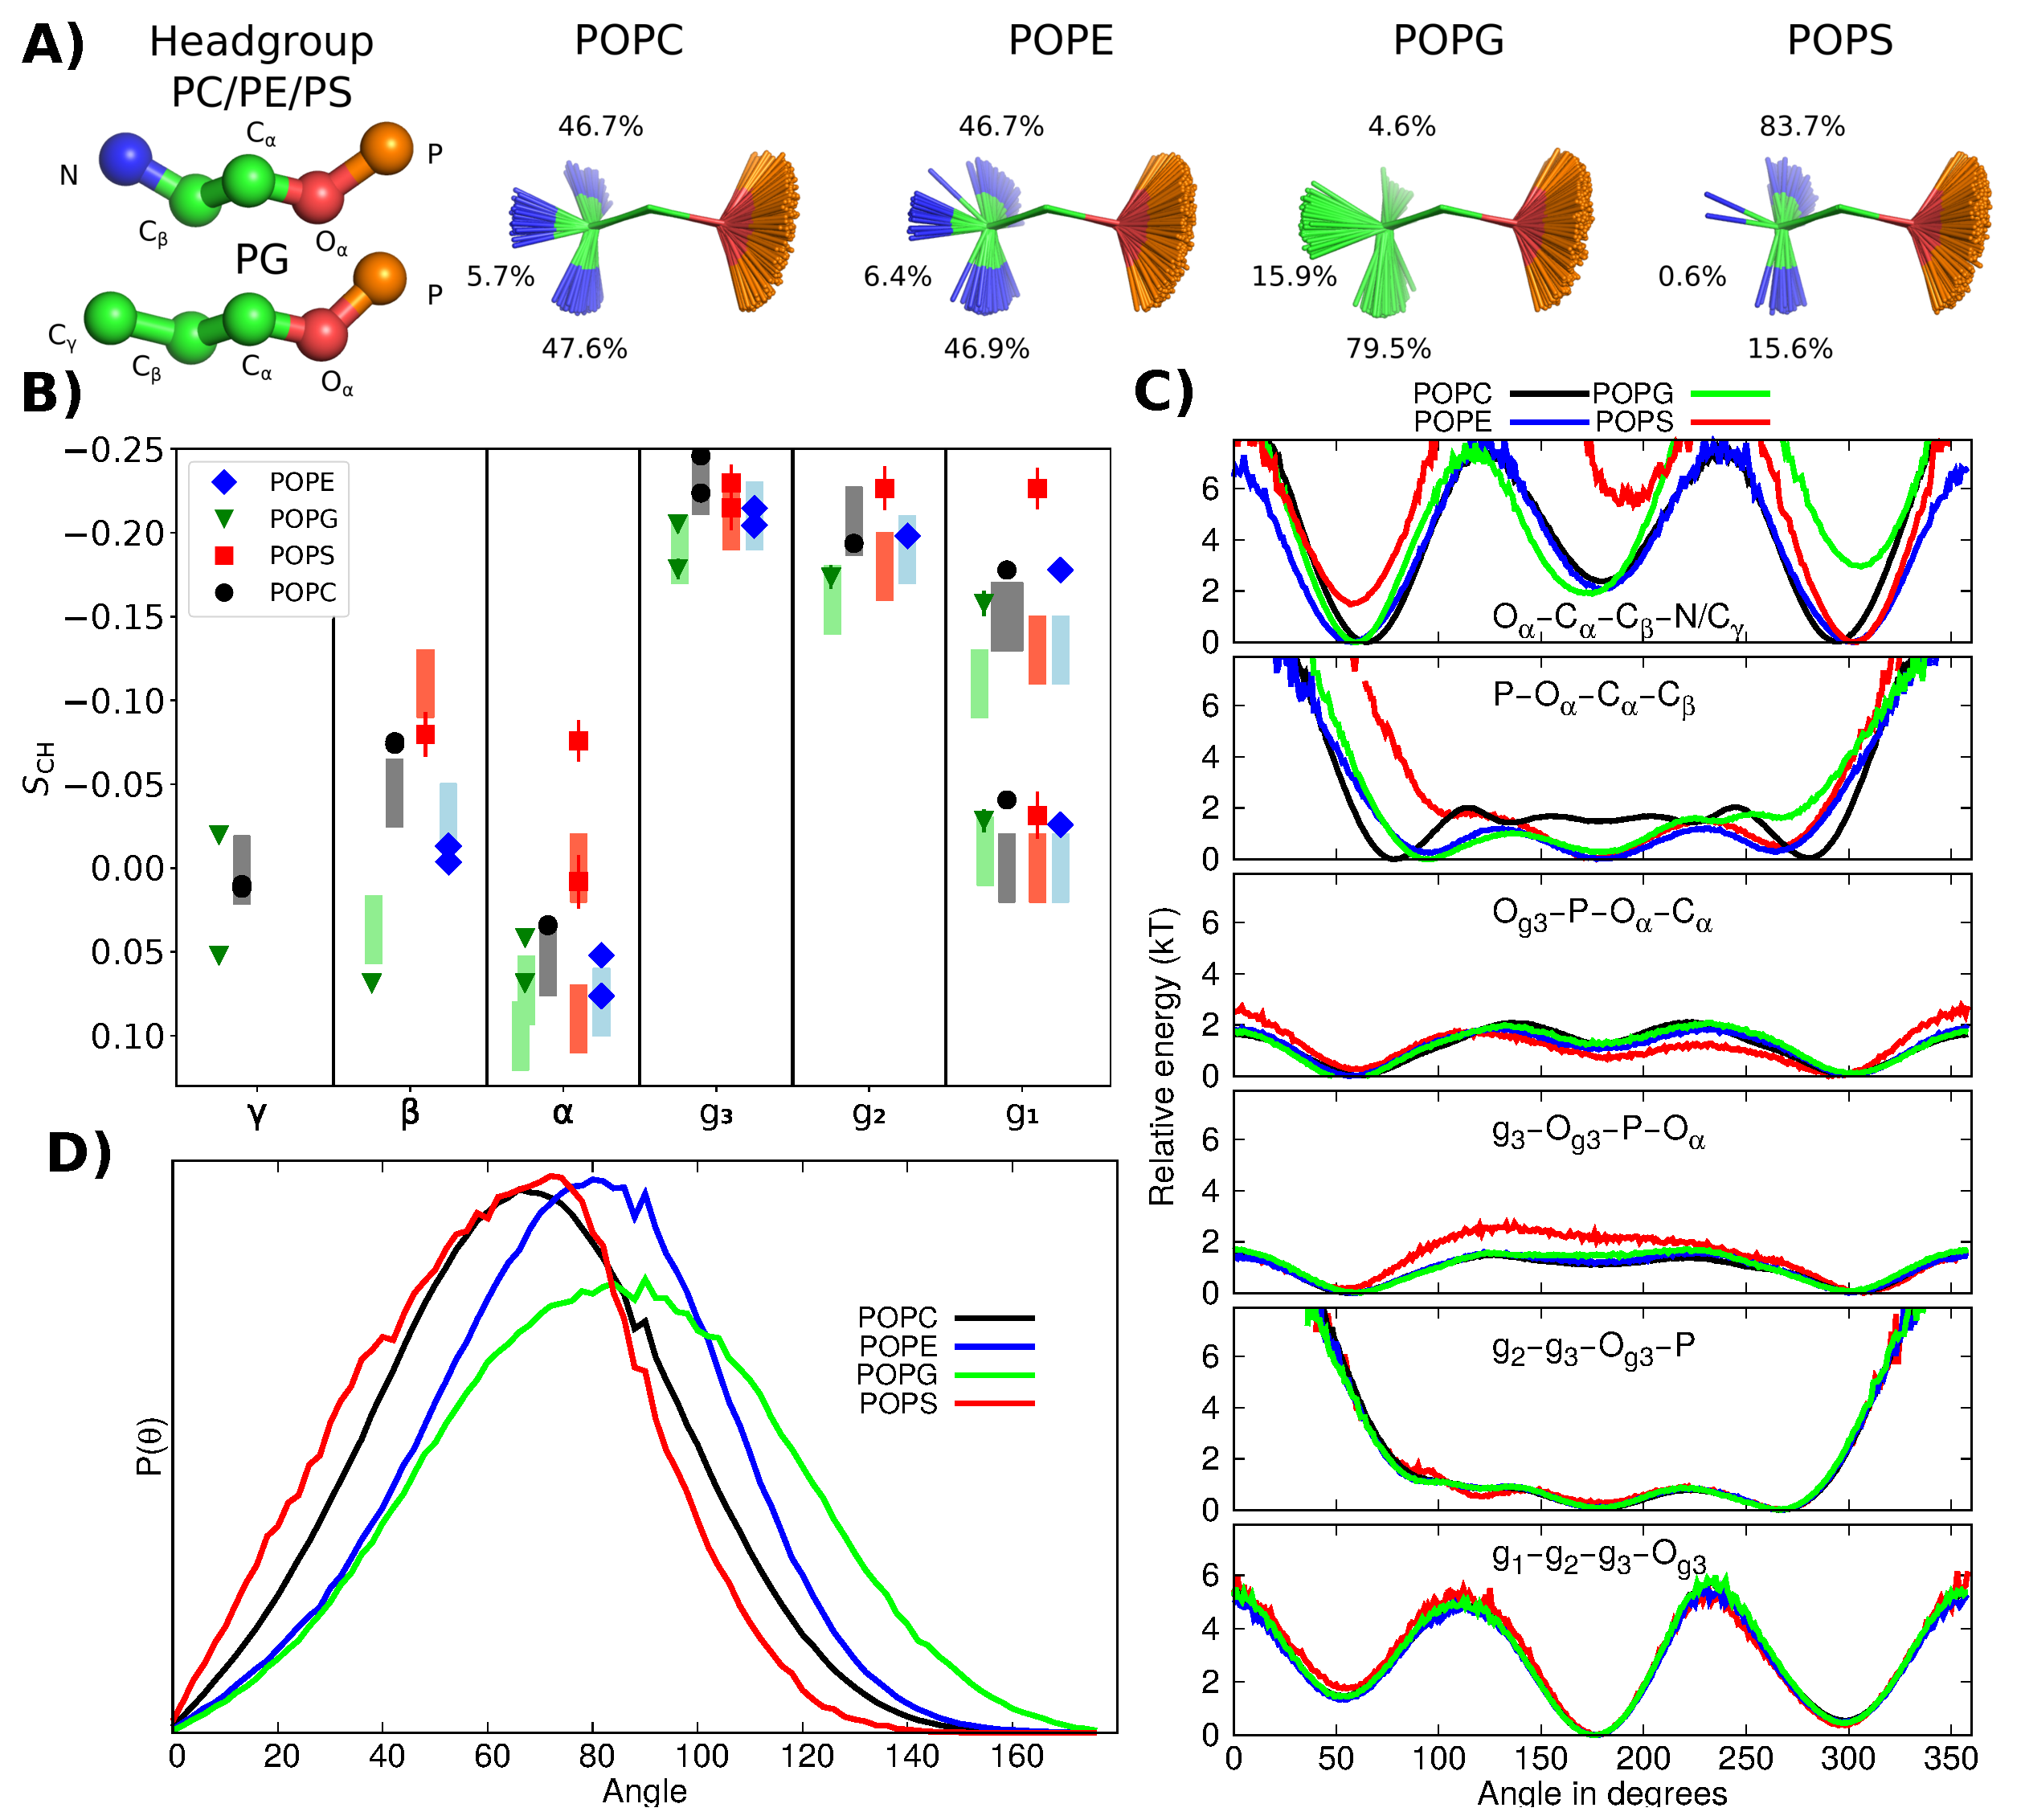
\includegraphics[width=18.0cm]{../Figs/figure2.eps}
%  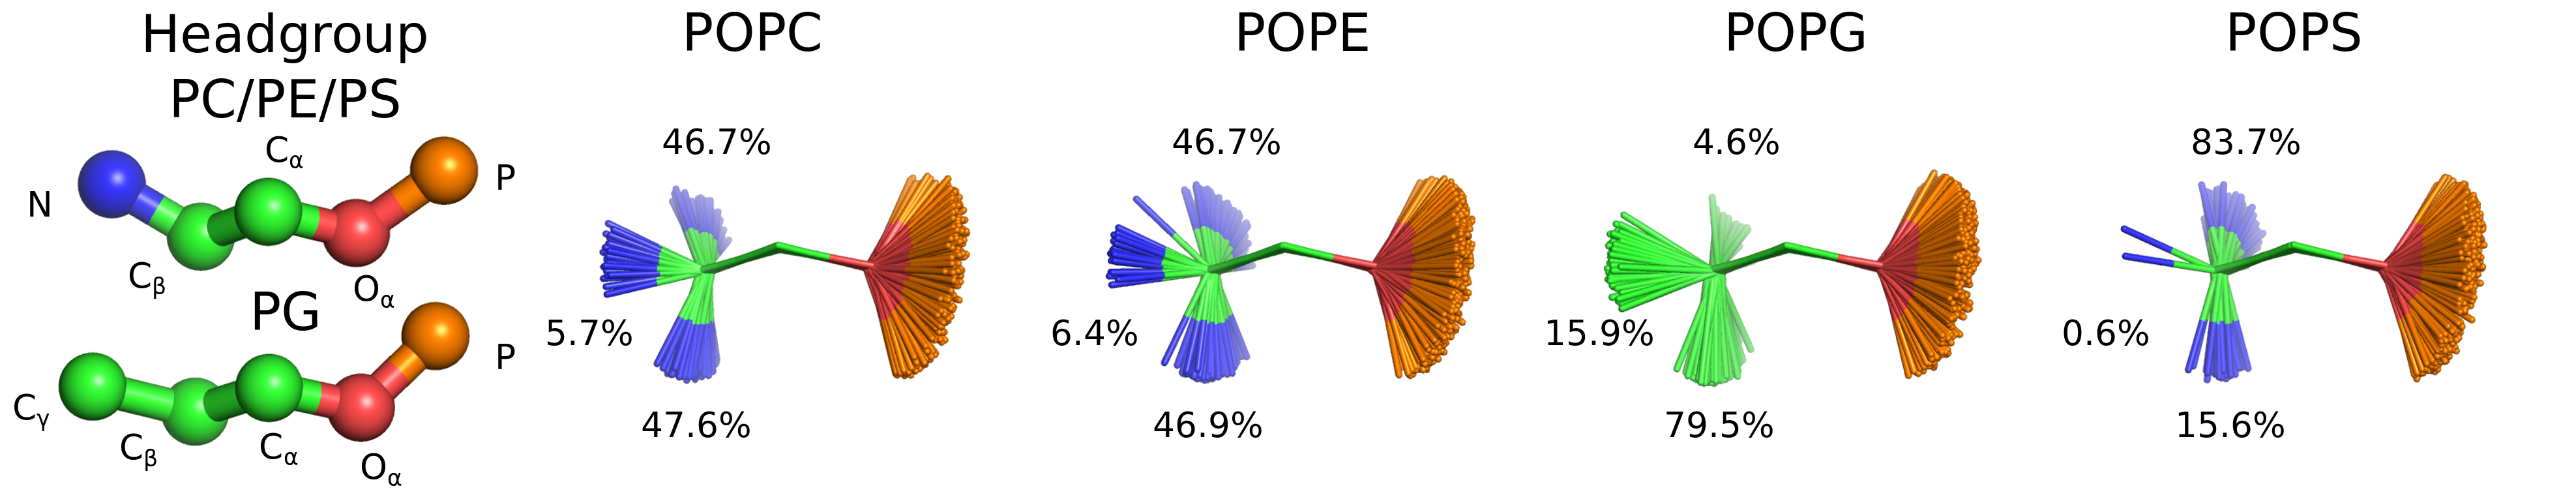
\includegraphics[width=18.0cm]{../Figs/PCPEPGPSstructures2.png}
%  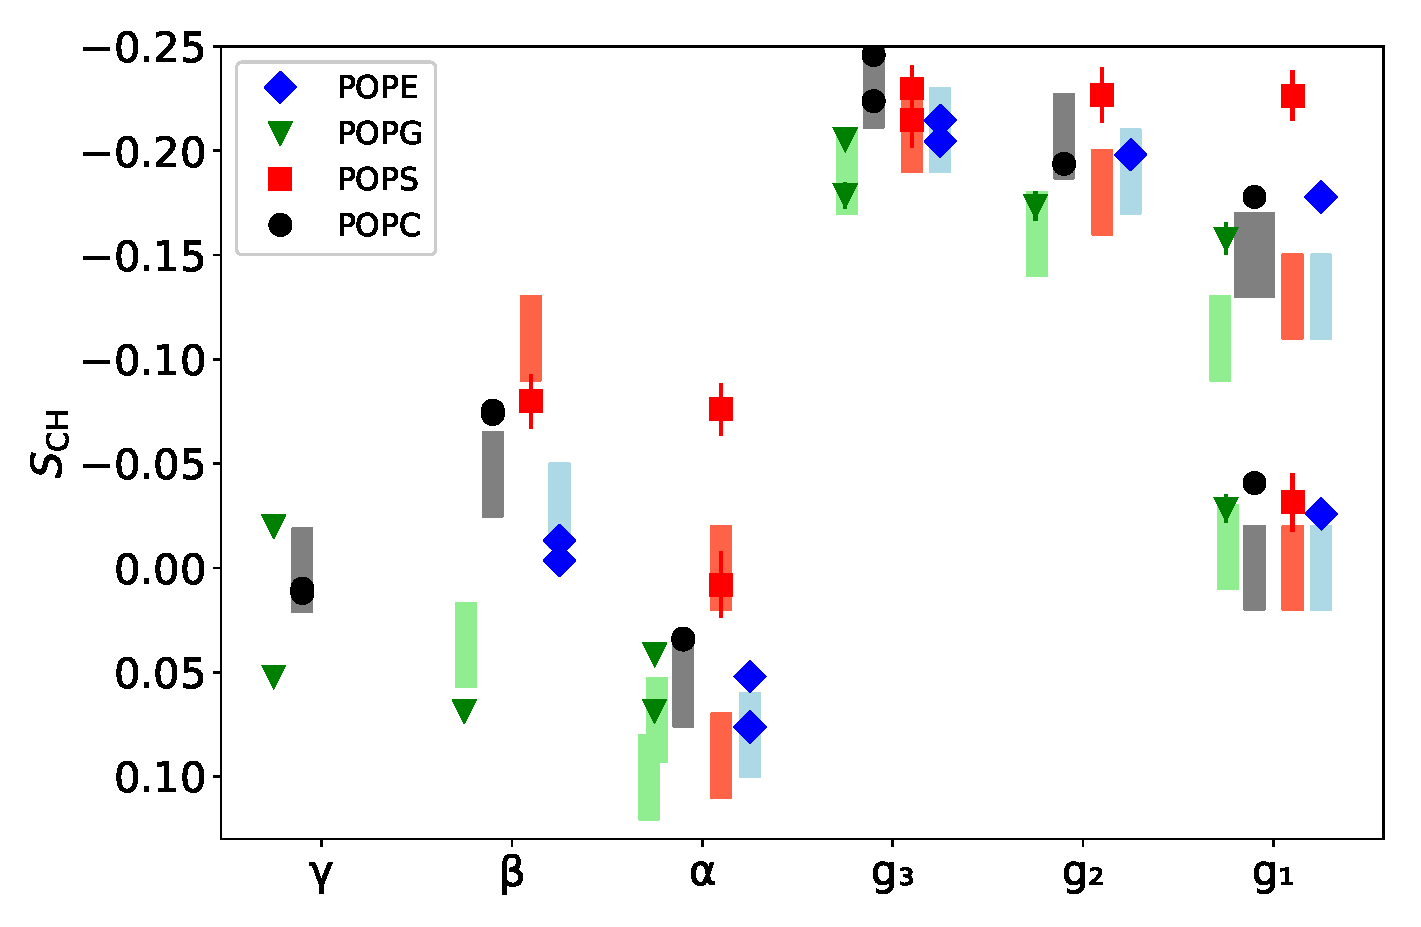
\includegraphics[width=8.0cm]{../Figs/CHARMMfromLIPIDS.eps}
%%  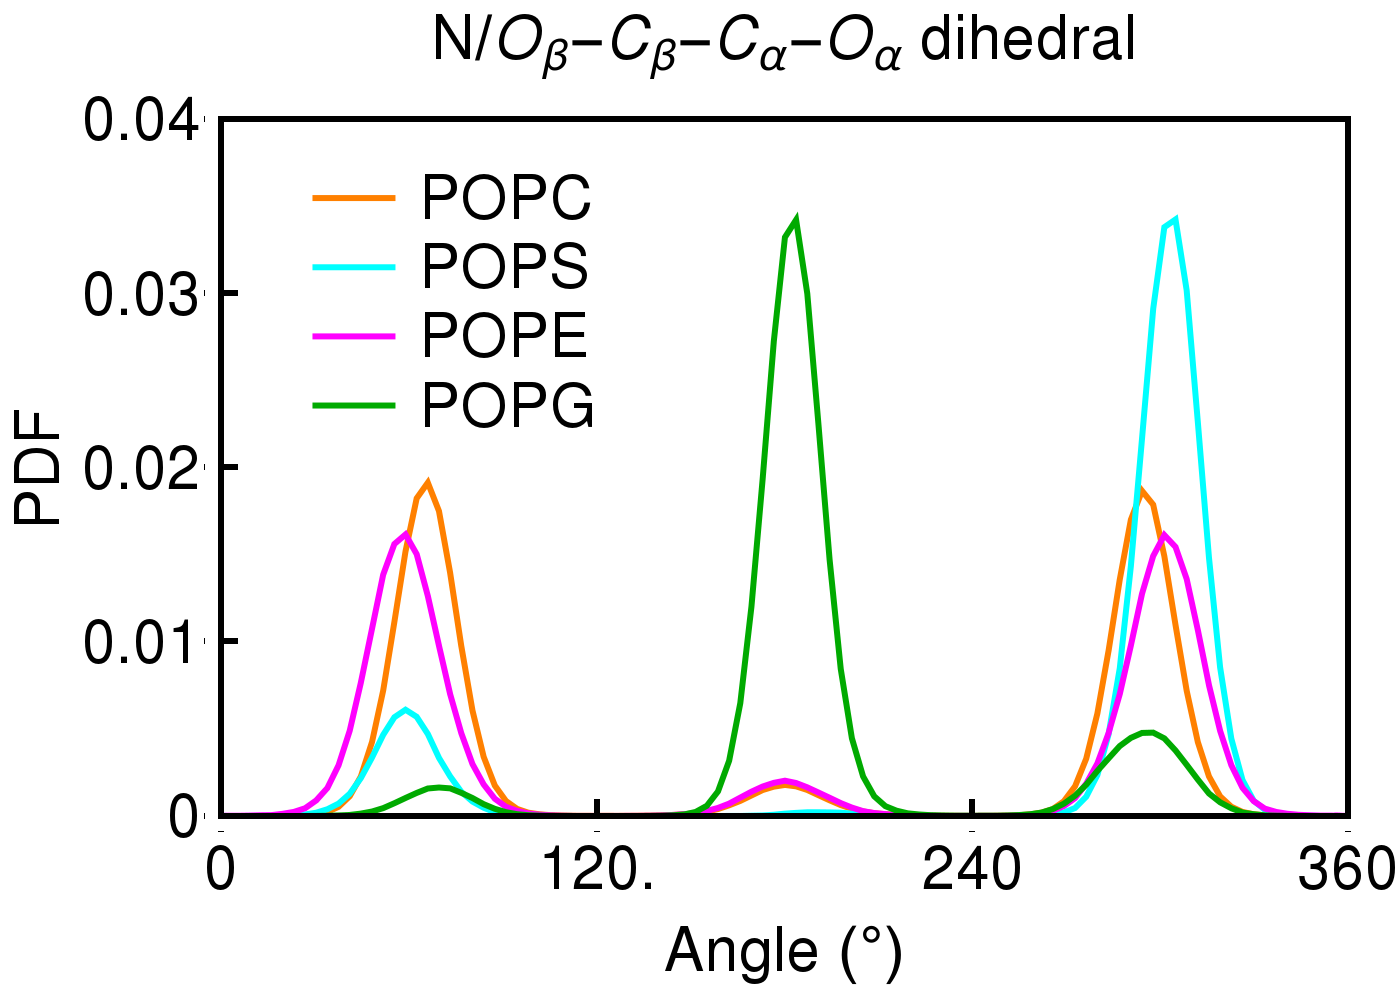
\includegraphics[width=8.0cm]{../Figs/PCPEPGPSdihedrals1.png}
%%  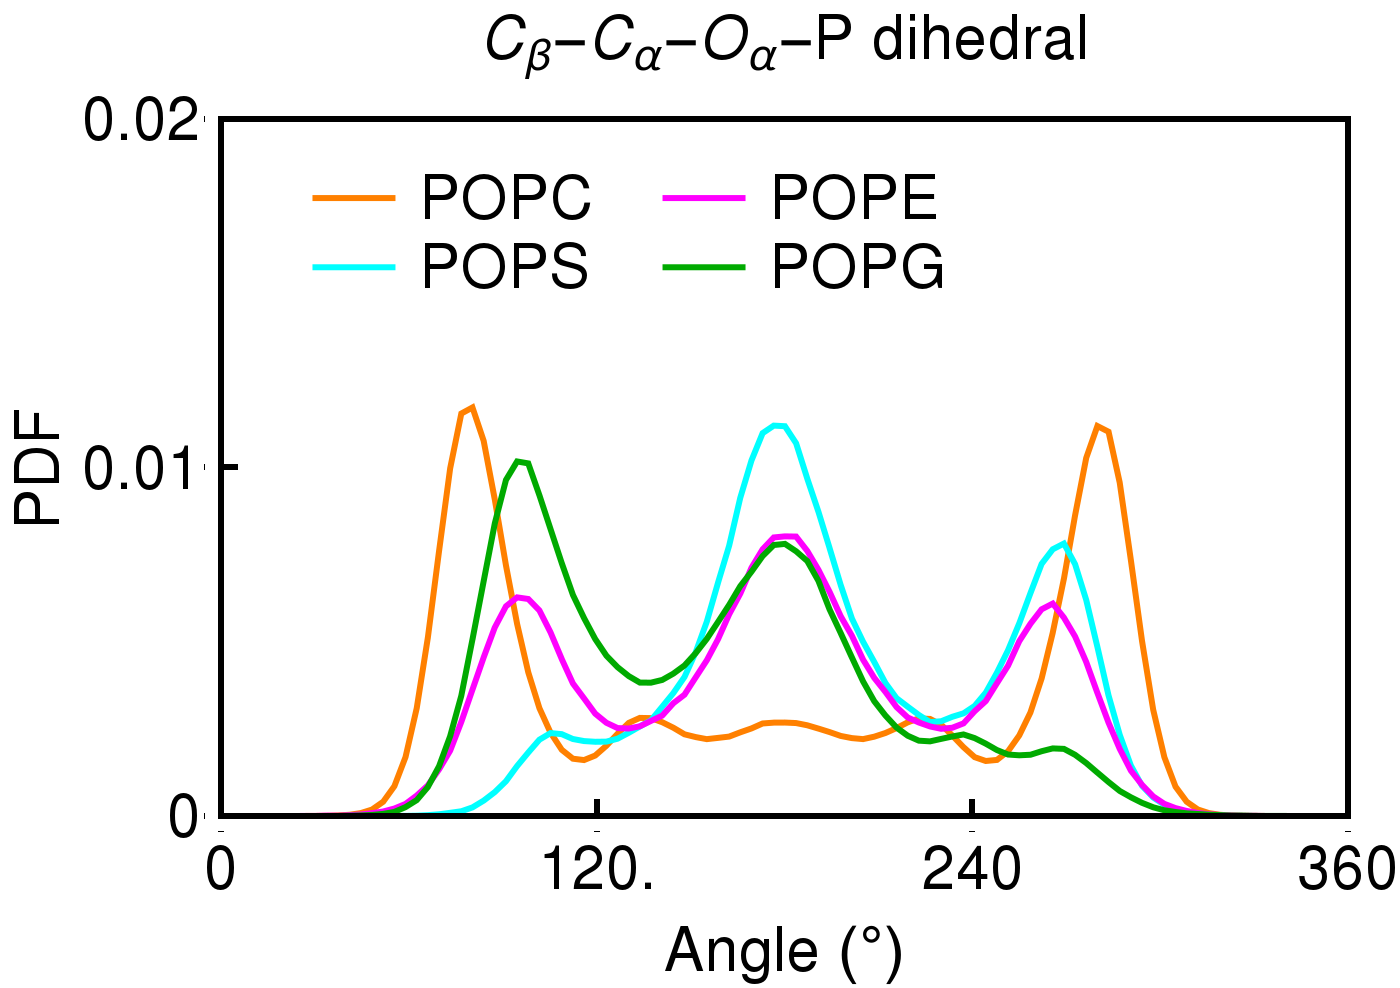
\includegraphics[width=8.0cm]{../Figs/PCPEPGPSdihedrals2.png}
%  \includegraphics[width=8.0cm]{../Figs/PNangleNORM.eps}
%  \includegraphics[width=8.0cm]{../Figs/DIHEDRALS.eps}
   \caption{\label{structures}
     Results from CHARMM36 simulations demonstrating the differences in conformational ensembles betwee different lipids. 
     {\bf A)} Snapshots with overlayed C$_\beta$, C$_\alpha$ and O$_\alpha$ atoms and occurence of different conformations.
     {\bf B)} Headgroup and glycerol backbone region order parameters of different different lipids.
     {\bf C)} Distributions of heavy atom dihedral angles of different lipids from CHARMM36 simulations.
     {\bf D)} Distributions of P-N vector angle with respect to membrane normal.
  }
  \todo{This is a draft and requires quite a bit of polishing.
    More detailed discussion of this figure is in https://github.com/NMRLipids/NMRlipidsIVPEandPG/issues/9} \\
\end{figure*}


\subsection{Conformational ensembles of different lipid headgroups in bulk bilayer}

To experimentally characterize the headgroup conformational ensembles of lipids
that are not bound to proteins in electrostatically neutral cell membrane,
we measured the C-H bond order parameters and their signs from of POPG and POPE
in liquid lamellar phase, as we did previously for POPC and POPS \cite{ferreira13,ferreira16,antila19}.
Determination of headgroup and glycerol backbone order parameters and their signs
was straightforward from the
%R-PDLF and S-DROSS
data in Figs. \ref{HGorderParameters}, \ref{POPEspectra} and \ref{POPGspectra}
for all the C-H bonds, except the $\beta$ and g$_2$ carbons in POPG.
These carbons have overlapping peaks in the INEPT spectra due to their similar chemical environments,
and only the magnitude of the larger order parameter could be determined from the R-PDLF spectra (Fig. \ref{HGorderParameters} B).
Nevertheless, based on previous $^2$H NMR measurements \cite{wohlgemuth80,gally81,borle85},
we assigned the larger order parameter to the g$_2$ carbon
%order parameter of $\beta$-carbon is expected to be clearly smaller than for 
and used the literature value for the $\beta$-carbon in SIMPSON simulations to determine the signs.
The decrease in the beginning of the S-DROSS curve suggests that the sign of larger g$_2$ order parameter
is negative and later increase suggests that sign of smaller $\beta$ order parameter is positive (Fig. \ref{HGorderParameters} (B)).
This interpretation is confirmed by SIMPSON calculations in Fig \ref{POPGsimpson}.
%using negative value for g$_2$ and positive value for $\beta$ order parameter (Fig. \ref{POPGsimpson}).
%The signs of these order parameters were solved using SIMPSON simulations to interpre the
%S-DROSS experiments in similar fashion as we did previously for PS lipids \cite{antila19}.


%Also the headgroup order parameters of PC lipids are close PE, althought the latter gives systematically
%slightly more positive values (Fig. \ref{HGorderParameters}).
% These could be explained with slightly larger temperature in PE measurements, except for the $\alpha$-carbon with the positive sign, for which the
% more positive value is farther away from zero.
%While the headgroup order parameters are similar for PC and PE lipids,
%PG and PS lipids exhibit distinct values in comparison with other lipids.


Experimental order parameters of POPC, POPE, POPG and POPS glycerol backbones and
headgroups from this and previous studies are collected in Fig. \ref{HGorderParameters} D),
where signs determined from $^{13}$C NMR experiments are used also for the $^2$H NMR data from the literature.
%The resulting order parameters are compared with our previously published results
%for POPC \cite{ferreira13,ferreira16} and POPS \cite{antila19} in figure \ref{HGorderParameters} D.
%Order parameters for POPE are in good agreement with previous $^2$H NMR experiments \cite{seelig76}
%and similar to our previous results for POPC \cite{ferreira16}.
Overall agreement of order parameters determined by different authors and different techniques
for same lipid headgroup is very good in here and previous studies \cite{botan15,ollila16,antila19},
suggesting that the observed differences between lipid types arise from differences in
headgroup chemistry rather than inaccuracies in experiments. 
The most distinct order parameters are observed for PS headgroups,
for which the $\alpha$-carbon order parameter exhibits significant forking
and the $\beta$-carbon has more negative value than in other lipids.
On the other hand, the $\beta$-carbon order parameter of PG headgroup
%the $\alpha$-carbon order parameter is similar to PE and PG, while
has positive sign in contrast to all the other lipids.
Notably, this has not been observed in traditional $^2$H NMR experiments,
%because absolute value of $\beta$-carbon order parameter is similar in PG, PE and PC lipids and
where only the absolute value of the order parameters are measured~\cite{wohlgemuth80,gally81,borle85}.
The glycerol backbone order parameters are similar for all the lipids, although they move slightly toward
positive values (closer to zero) in the order PC $<$ PE $<$ PS $<$ PG.
Essential differences between PC and PE headgroups are not observed.

%As discussed previously for PC and PS headgroups \cite{ollila16,antila19}, also 
%the headgroup and glycerol backbone order parameters of PE and PG are essentially independent of 
%acyl chain composition, and therefore manifest mainly headgroup chemistry (Fig. \ref{HGorderParameters}).

\begin{figure*}[bt]
  \centering
  \includegraphics[width=18.0cm]{../Figs/HGorderparametersPCvsSURFchangeDIHEDRALS.eps}
  \caption{\label{changesWITHsurf}
    {\bf A)} Modulation of PC headgroup order parameters and P-N vector angle upon addition of cationic surfactant
    from CHARMM36 simulations compared with experimental data \cite{??}.
    {\bf B)} Changes in PC headgroup conformational ensembles upon increasing amount of positive charge in bilayer,
    characterized by the heavy atom dihedral distributions, from CHARMM36 simulations.
  }
\end{figure*}



To resolve the conformational ensembles of lipid headgroups,
we compared the headgroup and glycerol backbone C-H bond order parameters
from different MD simulation force fields to the experimental data. 
None of the force fields reproduced the order parameters
within experimental accuracy for any of the lipids analysed in this work
(Figs. \ref{HGorderParametersPE} and \ref{HGorderParametersPOPG}) or in our previous studies \cite{botan15,antila19}.
%has least problems in
%reproducing the experimental lipid headgroup and glycerol backbone order parameters in different
%lipids \cite{botan15,antila19} (Figs. \ref{HGorderParametersPE} and \ref{HGorderParametersPOPG}).
Nevertheless, the CHARMM36 force field performs best for all the headgroups and
%Importantly, it captures the experimentally observed distinct order parameters for PS and PG headgroups (Fig. \ref{??}).
%To characterize the differences in lipid headgroup conformational ensembles
reproduces the distinct order parameters of PS and PG lipids (Fig. \ref{structures} B).
To understand the structural origin of these distinct order parameters,
we calculated the distributions of heavy atom dihedral angles from CHARMM36 simulations in figure \ref{structures} C).
%The dihedral distributions in figure \ref{structures} show significant similarity between different lipids for all the other
%bonds, except
Major differences between headgroups are observed only for the last two dihedrals
in the headgroup end,  O$_\alpha$-C$_\alpha$-C$_\beta$-N/C$_\gamma$ and P-O$_\alpha$-C$_\alpha$-C$_\beta$,
which prefer {\it gauche$^-$} conformations for PG and {\it gauche$^+$} for PS.
Rest of the dihedrals are similar between different lipids, with the exception of
%However, some dihedral angles of phosphorus-oxygen bonds are less likely for PS, which
small differences for PS lipids. Therefore we suggest that the main differences between
lipid headgroups leading to distinct order parameter occur in the choline part, while
also changes in phosphate region may contribute in PS lipids, which could also
explain the more rigid headgroup structures~\cite{browning80,buldt81}.
%These differences explaing the disctinct order parameters of
%PS and PG headgroups with respenct to the other lipids.
%The differences between lipids are reflected also to
Furthermore, the angle between headgroup dipole and membrane normal
decreases in the order of PG $>$ PE  $>$ PC  $>$ PS (Fig. \ref{structures} B)).
However, the differences between PC and PE in P-O$_\alpha$-C$_\alpha$-C$_\beta$ dihedral
and P-N vector dipole may be an artefacts as the $\beta$-carbon order parameter in PC
is too negative the CHARMM36 force field, thereby not being equal to the order parameter
in PE as observed in experiments \cite{botan15}.


%The eclipsed (0 or 360 degrees) are not present in any other dihedrals, and anti-eclipsed (120 or 240 degrees)
%are not present in C$_\alpha$-C$_\beta$ and g$_1$-g$_2$ bonds.


%Characteristic dihedral conformations in PS headgroup are asymmetric conformations
%preferring gauche 270$^\circ$ conformations in N-C$_\beta$-C$_\alpha$-O$_\alpha$ and
%%dihedral exhibits a more asymmetric angle distribution for PS, having largest probability being
%%in , than for the PC headgroup.
%C$_\beta$-C$_\alpha$-O$_\alpha$-P dihedrals. 
%In PG headgroup, the O$_\beta$-C$_\beta$-C$_\alpha$-O$_\alpha$ dihedral (corresponding N-C$_\beta$-C$_\alpha$-O$_\alpha$ dihedral in other% lipids)
%is mostly in trans conformation, and C$_\beta$-C$_\alpha$-O$_\alpha$-P  has asymmetric tendency to be in
%gauche 60$^\circ$ conformation. 
%Main difference between PC and PE is the lower probability of trans state in C$_\beta$-C$_\alpha$-O$_\alpha$-P PC dihedral,
%which could be a potential reason for the too negative $\beta$ headgroup order parameter in PC.%


In conclusion, all lipid headgroups sample very broad conformational ensembles in liquid lamellar phase.
%the results suggest that free rotations around O-P bonds decouple the
%headgroup and glycerol backbone structure and dynamics in similarly in all lipids,
%althought this rotation is slower in PS lipids where crossing certain barriers are slower.
Despite the differences in distributions
%of two the last bonds at the headgroup end,
%leading to the distinct order parameters for PS and PG lipids,
%lipids with
between headgroups, the sampled dihedral angles are within approximately same ranges for all headgroup types.
Therefore, we suggest that all lipid headgroups are very flexible thereby being
able to adopt wide range of multiple conformations when interacting with proteins, ions or other biomolecules.
%Furthermore, approximately same conformations are present liquid lamellar phase for different
%headgroups studied here, althought the probability weight for the conformations are slightly different.
%the order parameter experiments suggest that the glycerol backbone conformations in all lipids
%and the headgroup conformations in PC and PE lipids are relatively similar, while 
%PS and PG headgropus exhibit distinct conformational sampling.
%The details of sampled conformation are difficult to deduce from order parameters only,
%but the distinct headgroup order parameters
%of PS lipids are previously related to the more rigid structure of the headgroup~\cite{browning80,buldt81,antila19}.
%The analysis of dihedral angle distributions reveal the free rotation of dihedral around
%phosphorus-oxygen bonds in all lipids as all possible angles are observed in the distributions.
Our results support the models that propose free rotation around phosphate group for PC lipids,
which decouples the dynamics and conformatios between acyl chains and headgroups \cite{klauda08c,antila21b},
and suggests that these models could be applied for all lipids containing the phosphorus group.
The wide range of observed conformations suggest that the structures in lipid crystals \cite{buldt81,pascher92}
play only a minor role, and that the models aiming to explain NMR data using only few conformations \cite{seelig77c,davis83,Semchyschyn04,akutsu20}
are not sufficient to capture the large conformational space of lipids in liquid lamellar state.


\subsection{Lipid conformational ensembles in lipid bilayers with bound ions}

Charged lipids, proteins, surfactants, drugs, and ions incorporated in membranes
reorient the headgroup dipole in PC lipids, thereby affecting the order parameters of
lipid headgroups \cite{seelig87}. However, detailed understanding on
lipid conformational ensembles in membranes bearing electric charge is still lacking \cite{Semchyschyn04}.
%Order parameters of $\alpha$ and $\beta$ carbons in PC lipid headgroup are known to depend
%linearly on the incorporation of charged molecules into a lipid bilayer,
%which is explained by tilting of the headgroup dipole orientation \cite{??}.
%%are kn affect the headgroup dipole vector tilt which can
%%be detected by measuring C-H bond order parameters of $\alpha$ and $\beta$ carbons.
%Such changes have been observed upon addition of charged lipids, proteins, surfactants,
%drugs, or ions \cite{??}, but how charges affect the lipid conformational ensemble remains unknown.

\begin{figure*}[]
  \centering
  \includegraphics[width=18.0cm]{../Figs/CHANGESwithCaClPG1PC1.eps}
  \caption{\label{changesWITHCaClPG}
    Modulation of headgroup order parameters of POPC ({\it left}) and POPG ({\it right}) in POPC:POPG (1:1)
    mixture upon addition of CaCl$_2$ in 298 K temperature from experiments \cite{borle85,macdonald87} and simulations.
    The $\beta$-carbon order parameter of POPC (dashed line on top left) is not directly measured but
    calculated from empirical relation $\Delta S_{\beta}=0.43\Delta S_{\alpha}$ \cite{akutsu81}.
    The changes with respect to the systems without CaCl$_2$ are shown for other data than
    for the $\alpha$-carbon of POPG for which experimental order parameter is not available.
    Calsium density distributions are shown in figure \ref{CAdensPG}.
    %(right) The headgroup order parameters of PG from PC:PG mixtures as a function CaCl$_2$
    %concentration from experiments \cite{borle85} and CHARMM36 simulations.
  }
\end{figure*}


To resolve lipid headgroup conformational ensembles in cell membrane bearing positive charge,
%suggesting that these simulations can be used to interpret the charge induced changes in lipid conformational ensembles.
we first analyzed CHARMM36 simulations which correctly captures the experimentally measured decrease in PC headgroup order parameters
upon addition of cationic surfactants into a bilayer in figure \ref{changesWITHsurf} A).
Heavy atom dihedral angle distributions in figure \ref{changesWITHsurf} B
reveal that the decrease of trans state probabilities in g$_2$-g$_3$-O$_{g_3}$-P and g$_3$-O$_{g_3}$-P-O$_\alpha$
dihedrals are the major effects of positive charge on lipid headgroup conformations.
Choline region remains essentially unchanged and only minor changes are observed in other dihedrals
even thought almost half of the molecules in membranes are cationic surfactants.
%The major changes upon addition of charge are observed in dihedrals related to the phosphate oxygens,
%while small change is observed also in the g$_2$-g$_3$ bond in the glycerol backbone.
%This result is in line with the recently proposed model suggesting that the flexible phosphate enables the headgroup
%orient according to the charge accumulated into a membrane \cite{antila21}.
We also tried to resolve PC lipid headgroup conformational ensembles in mixed membrane with
negatively charged lipids \cite{scherer87},
%Headgroup order parameters of PC lipids respond similarly also to the addition of charged lipids in experiments \cite{??}.
%To resolve the conformational ensembles of lipid headgroups also in biologically relevant
%mixtures, % of zwitterionic and charged lipids,
%we compared the response of headgroup order parameters in
%PC lipids to the addition of PE or PG (Fig. \ref{??}),
%as well as in PG lipids to the addition of PC (Fig. \ref{??}),
%between simulations and experiments. However, the
but the accuracy of currently available force fields
was not sufficient for this (Fig. \ref{HGorderparametersPCvsPEPG}).
%to capture the headgroup conformational ensembles
%in mixed membranes: 
%The best performing force field for single componen membranes, CHARMM36, overestimates
%the effect of PE to PC conformations and underestimates the response PC to the addition
%of anionic PG headgroup. Previously we explained similar result for PC/PS mixtures  
%%as we previously observed also for mixtures with PS lipids \cite{antila19}.
%%The latter may arise from
%by overbinding of the sodium counterions \cite{antila19}.


Also binding of ions may affect the lipid headgroup conformational ensembles in physiological conditions.
The resolve this effect, we compared the changes of headgroup order parameters
in POPC:POPG mixtures 
upon addition of CaCl$_2$ between different simulations and experiments \cite{borle85,macdonald87}
in figures \ref{changesWITHCaClPG} (molar ratio 1:1) and \ref{changesWITHCaClPG1PC4} (molar ratio 4:1).
The results are in line with our previous studies:
most force fields overestimate the calcium binding \cite{catte16,antila19}, but CHARMM36 with the NBfix correction
underestimates the binding affinity \cite{antila19}, and the implicit inclusion of electronic polarizability
using the electronic continuum correction (ECC) improves the results \cite{melcr18,melcr20}.
The most realistic response of PC lipid headgroup order parameters to the calcium binding
is observed in the Lipid17ecc simulations with the ECC included, where
the decreased probability for trans state of g$_3$-O$_{g3}$-P-O$_\alpha$ dihedral
is the main structural consequence of bound ions (Fig. \ref{DIHSwithCAlipid17eccPOPC}).
Similar but smaller effect is seen in CHARMM36 simulations with less bound calcium (Fig. \ref{DIHSwithCAcharmm36POPC}).

%distribution from
%to eclipsed conformations 
%In this model, the main effect of calcium to the lipid conformational ensemble is
%the slight change of 
%This is in line with the changes observed in CHARMM36 simulations upon addition of charged surgactants (Fig. \ref{changesWITHsurf}),
%despite the major differences in lipid headgroup conformational ensembles between
%these models without ions (Fig. \ref{structures} vs. Fig. \ref{DIHSwithCAlipid17eccPOPC}).


%of lipid headgroup is not 
%Changes in lipid conformational ensembles characterized by distributions of heavy atom dihedral angles
%are very small upon binding of calcium or addition of cationic surfactants to membranes (Figs. \ref{??}).
%Yet, such changes are sufficient to tilt the headgroup dipole angle and reproduce the experimentally observed
%order parameter changes in $\alpha$ and $\beta$ carbons. 


%Among the available simulations, there are two models that correctly reproduce the
%PG headgroup order parameter changes upon addition of calcium, Lipid17 and Slipids,
%even though the binding affinity of calcium is overestimated in these simulations.
%The response of PC to calcium binding is correctly reproduced by Lipid17ecc model, as
%previously reported for other membranes \cite{melcr18,melcr19}.



%to Amber based lipid models
%improves the ion binding affinity leading to a good agreement with experiments.
%(Figs. \ref{changesWITHCaClPG} and \ref{changesWITHCaClPG1PC4})
%
%indicating too strong binding affinity of calcium into the bilayers as previously
%observed for pure PC lipid bilayers and mixtures with PS lipids \cite{catte16,antila19}.
%
%The decrease of $\alpha$-carbon order parameter of PC lipids in PC:PG mixtures as a function
%of calcium concentration is close to experiments CHARMM36 simulations (Fig. \ref{changesWITHCaClPG}),
%but the decrease of $\beta$-carbon order parameter seems to be overestimated.
%However, the $\beta$-carbon order parameter was not actually measured from these samples,
%but they are calculated from empirical relation $\Delta S_{\beta}=0.43\Delta S_{\alpha}$ \cite{akutsu81}.
%On the other hand, the simulations are not converged.
%
%The calcium binding affinity to lipid bilayers with PC and PS lipids
%was recently improved by applying the electronic continuum correction (ECC) to Amber Lipid14/17 force fields \cite{melcr18,melcr20}.
%In this approach, the electronic polarizability is implicitly included in the classical force fields
%by scaling the charges with constant factors \cite{leontyev11}. Here, we make a ECC-POPG force field
%by applying the scaling factors originally used for POPS also to POPG, i.e., we multiply
%charges and Lennard-Jones $\sigma$s of headgroup, glycerol backbone, and carbonyl regions with 
%$f_q$=0.75 and $f_\sigma$=0.89, respectively \cite{melcr20}.
%ECC-POPG model gives a weaker calcium binding affinity (Fig.\ref{CAdensPG}) and better agreement with the experimental
%PC headgroup order parameter changes (Fig. \ref{changesWITHCaClPG}) for POPC:POPG mixtures than the original Lipid17 model
%\todo{to be finished when we have all the data}, indicating that the ECC improves the simulation predictions of
%calcium binding affinity as previously observed for PC and PS lipids \cite{melcr18,melcr20}.



%\begin{figure}[]
%  \centering
%  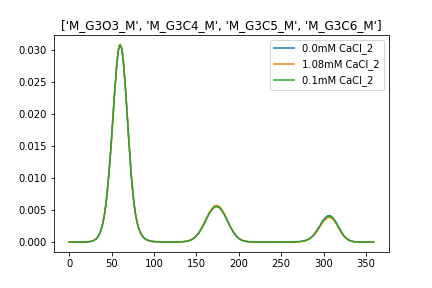
\includegraphics[width=6.0cm]{../Figs/dihedralFIGS/POPG_M_G3O3_M_M_G3C4_M_M_G3C5_M_M_G3C6_MCHARMM36.png}
%  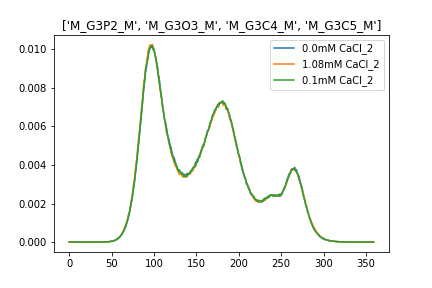
\includegraphics[width=6.0cm]{../Figs/dihedralFIGS/POPG_M_G3P2_M_M_G3O3_M_M_G3C4_M_M_G3C5_MCHARMM36.png}
%  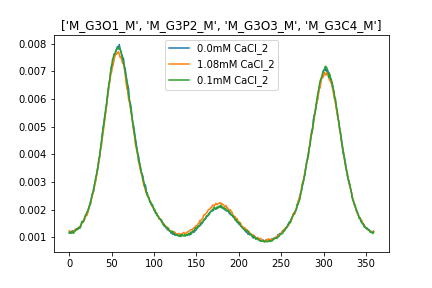
\includegraphics[width=6.0cm]{../Figs/dihedralFIGS/POPG_M_G3O1_M_M_G3P2_M_M_G3O3_M_M_G3C4_MCHARMM36.png}
%  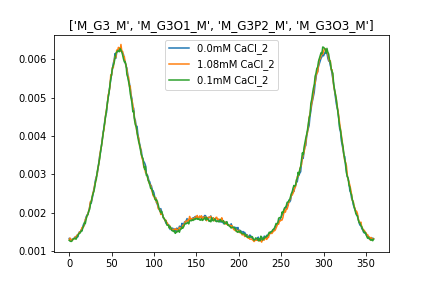
\includegraphics[width=6.0cm]{../Figs/dihedralFIGS/POPG_M_G3_M_M_G3O1_M_M_G3P2_M_M_G3O3_MCHARMM36.png}
%  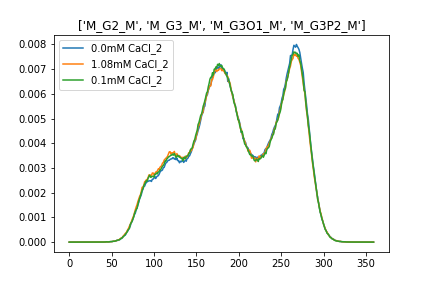
\includegraphics[width=6.0cm]{../Figs/dihedralFIGS/POPG_M_G2_M_M_G3_M_M_G3O1_M_M_G3P2_MCHARMM36.png}
%  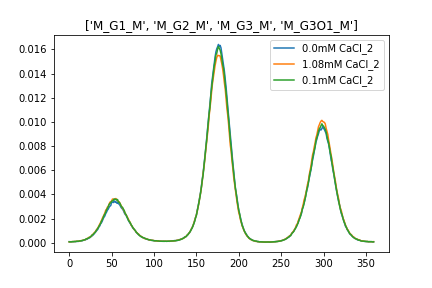
\includegraphics[width=6.0cm]{../Figs/dihedralFIGS/POPG_M_G1_M_M_G2_M_M_G3_M_M_G3O1_MCHARMM36.png}  
%  \caption{\label{DIHSwithCA}
%    Changes in POPG CHARMM36 dihedrals with increasing amount of CaCl$_2$.
%  }
%\end{figure}

%Simulations also qualitatively reproduce the experimentally observed decrease of POPG
%%Experimental data for the
%$\beta$-carbon order parameter
%%of POPG shows a rapid decrease with increasing
%upon addition of CaCl$_2$,
%%concentrations up to 10 mM
%suggesting that the PG headgroup response is qualitatively captured by simulations, in contrast
%to PS in our previous work \cite{antila19}.
%and more modest decrease with larger concentrations (Fig. \ref{changesWITHCaClPG}) \cite{borle85}.
%This behaviour is similar to that of $\beta$-carbon order parameters of POPC,
%but essentially different than observed for POPS, where $\beta$-carbon order parameters increases with
%addition of calcium \cite{antila19}. Experimentally measured changes of PG $\alpha$-carbon order parameters upon addition of
%calcium are not available.
%%upon addition of calcium in experiments,
%%exhibiting 
%%The behaviour is qualitatively different than in the $\beta$-carbon of PS lipids which increase upon addition of CaCl$_2$.

%Decrease in headgroup order parameters of PC lipids upon addition of charges is
%usually qualitatitely captured in simulations despite the inaccuries in lipid conformational ensembles \cite{catte16},
%but situation with PS lipids is more complicated \cite{antila19,melcr20}.
Also the headgroup order parameters of charged lipids are affected by the binding of ions,
but their response is less well understood and more difficult to capture in MD simulations \cite{antila19,melcr20}.
In our simulations, the Lipid17 and Slipids force fields give the most realistic response of PG $\beta$-carbon to CaCl$_2$
in figure \ref{changesWITHCaClPG} even thought the calcium binding affinity was overestimated in these models.
%Even thought the
%change in headgroup orientation upon addition of calcium is smaller
%On the other hand, the
These models suggest that the upward tilting of the headgroup dipole is weaker in PG than in PC headgroup (\ref{changesWITHCaClPG}),
%Heavy atom dihedral angle distributions calculated from these simulations
%suggest that also the headgroup glycerol conformations in PG are affected by calcium
but dihedral distributions are more sensitive to the bound ions in PG 
(Figs \ref{DIHSwithCAslipidsPOPG} and \ref{DIHSwithCAlipid17POPG}).
%in contrast to PC lipids where only conformations near phosphate were affected.
%, possible due to the compensating effects from the changes in
%phosphate and glycerol regions. 
However, none of the simulations captures the calcium binding affinity and conformational ensemble of PG lipids
simultaneously, experimental data to evaluate the response of $\alpha$-carbon order parameters to
the added calcium in PG is not available, and changes in dihedrals upon addition of cacium differ between
the best models (Figs \ref{DIHSwithCAslipidsPOPG} and \ref{DIHSwithCAlipid17POPG}).
Therefore, more accurate force fields are required for the detailed analysis of the interactions between ions
and charged lipids, as concluded previously also for PS lipids \cite{antila19,melcr20}.

%and PG
%The response of PG $\alpha$-carbon order parameters to CaCl$_2$ differs between force fields,
%but experimental data to evaluate these predictions is not available. 
%Simulations also qualitatively reproduce the experimentally observed decrease of POPG
%%Experimental data for the
%$\beta$-carbon order parameter
%%of POPG shows a rapid decrease with increasing
%upon addition of CaCl$_2$,
%%concentrations up to 10 mM
%suggesting that the PG headgroup response is qualitatively captured by simulations, in contrast
%to PS in our previous work \cite{antila19}.
%and more modest decrease with larger concentrations (Fig. \ref{changesWITHCaClPG}) \cite{borle85}.
%This behaviour is similar to that of $\beta$-carbon order parameters of POPC,
%but essentially different than observed for POPS, where $\beta$-carbon order parameters increases with
%addition of calcium \cite{antila19}. Experimentally measured changes of PG $\alpha$-carbon order parameters upon addition of
%calcium are not available.
%%upon addition of calcium in experiments,
%%exhibiting 
%%The behaviour is qualitatively different than in the $\beta$-carbon of PS lipids which increase upon addition of CaCl$_2$.


% The result is similar to the $\sim$200~ns simulations with PC lipids in previous work \cite{catte16}.
%However, when simulation was continued for $\mu$s, the binding affinity substantially increased
%and interpretation was that calcium overbinds to PC lipid in CHARMM36. Therefore, the
%conclusion seems to be similar here, although the new NBfix parameters may complicate
%the situation \todo{The status of NBfix parameters in these simulations should be checked.}.

%The $\beta$-carbon order parameter of PG exhibits a rapid decrease with small CaCl$_2$ concentrations
%and a more modest decrease with larger concentrations in experiments \cite{borle85} (Fig. \ref{PSPGchangesWITHCaCl}).
%The rapid decrease with CaCl$_2$ is observed but overestimated in CHARMM36 simulation
%with POPC:POPG 1:1 mixture, but not in 4:1 mixture \todo{This is little bit weird, should be checked.}.

%\todo{We still need more data to finish the discussion. More detailed discussion is in https://github.com/NMRLipids/NMRlipidsIVPEandPG/issues/12}

Despite the limited capability of simulations to interpret some of the experimental data due to
the inaccuries in force fields, we conclude that the experimentally observed changes
in headgroup order parameters upon addition of charges into bilayer arise from relatively
small changes in conformational ensembles. These changes eventuate from
mild changes in dihedral angle distributions, rather than from restriction of lipids into
fixed conformations. Therefore, lipid headgroups remain in disordered state sampling large
space of different conformations, thereby being able to interact with different molecules
in various ways, also in membranes bearing electric charge.



\subsection{Protein bound lipid conformations}

To analyze lipid conformations in protein bound states,
we calculated the heavy atom dihedral distributions from 
all lipid conformations available within protein structures
deposited in the PDB \cite{berman00} in figure \ref{dihedralsFROMpdb}.
We found 176 PC, 198 PE, 70 PG, and 41 PS conformations, which
present lipids that are tightly bound to proteins in fixed conformations
that can be determined as a part of protein structure using crystallography, NMR, or cryo-EM. 


\begin{figure}[]
  \centering
  \includegraphics[width=8.0cm]{../Figs/DIHEDRALSALLfromPDB.eps}
%  \includegraphics[width=8.0cm]{../Figs/DIHEDRALSPEfromPDB.eps}
%  \includegraphics[width=8.0cm]{../Figs/DIHEDRALSPGfromPDB.eps}
%  \includegraphics[width=8.0cm]{../Figs/DIHEDRALSPSfromPDB.eps}
  \caption{\label{dihedralsFROMpdb}
    Dihedral distributions from simulations and lipid structures in PDB.
  }
\end{figure}

Similarly to the liquid lamellar state, lipid dihedrals have very wide range of angles
when bound to proteins. Only %restrictions seem to be in 
%Almost all dihedral angles are found from the protein bounds states for all dihedrals
%except for
P-O$_\alpha$-C$_\alpha$-C$_\beta$ and g$_2$-g$_3$-O$_{g_3}$-P dihedrals
seem to avoid cis conformations as observed also in liquid lamellar state.
The %range of available angles for
O$_\alpha$-C$_\alpha$-C$_\beta$-N/C$_\gamma$ and
g$_1$-g$_2$-g$_3$-O$_{g_3}$ dihedrals are even less restricted in protein bound state
than in liquid lamellar phase where cis and anti ecplipsed state were not present (Fig. \ref{structures}). 
Major differences between different lipid headgroups are not observed when bound to proteins.
Slight preference for the trans state in O$_\alpha$-C$_\alpha$-C$_\beta$-/C$_\gamma$ dihedral of PC,
and for positive angles in P-O$_\alpha$-C$_\alpha$-C$_\gamma$ dihedral of PS lipids with respect
to other lipids could be present in the data, but the statistics is not sufficient for conclusions.
Therefore, the differences in conformational ensembles between different
lipids in liquid lamellar state in Fig. \ref{structures} are not seen in the protein bound states.

This suggests that lipids can bind to proteins in wide range of conformations independently
of headgroup chemistry. Thereby, lipids compromize their preferred conformations when binding
to proteins and the binding of lipids to specific locations would be driven by 
the intermolecular interactions between proteins and lipids.
However, it is important to note that lipids are often not the main target in
structures deposited in PDB and therefore their conformations may be less reliable than proteins.
Stereochemical violations and structures deviating from lipid crystals have been
previously proposed to indicate inaccuracies in lipid structures in PDB \cite{marsh13b,pezeshkian18}. 
However, we see large deviations from lipid crystals structures also in conformational ensembles
that reproduce the NMR data in liquid lamellar phase, thereby proposing that such deviations
are realistic also in protein bound states.

\section{Conclusions}

%We have measured the C-H bond order parameters with the signs for headgroup and glycerol
%backbone regions of the
Conformational ensembles resolved using solid state NMR experiments and MD simulations
from NMRlipids open collaboration revealed that headgroups of the most abundant biological
phopholipids, PC, PE, PG and PS, sample wide range of different conformations in lamellar liquid state.
%Combining this experimental data with the large amount of simulation data collected 
%using the NMRlipids open collaboration, we were able to resolve the differences between
%conformational ensembles of lipid headgroup leading to the differences observed in NMR experiments.
%Our results indicate that lipid headgroups are flexible and sample large conformational space
%in biologically relevant liquid lamellar state,
Differences in NMR order parameters between different headgroups can be explained
by the changes in dihedral angle distributions, suggesting that
similar conformations are accessed by all headgroups, but with different probabilities.
Also the changes in order parameters upon addition of charged molecules, such as cationic lipids, surfactants, or drugs,
in membranes can be explained by the changes in dihedral angle probabilities, particularly close to the phosphate region.

Wide range of conformations are observed also in lipids that are tightly bound to proteins in PDB,
%Therefore, lipids can bind to proteins and other biomolecules in multiple different conformations,
%as indeed observed in the analysis of protein bound lipid conformations available from PDB.
%The weak correlation between lipid structures in liquid lamellar phase and protein bound state
suggesting that the specific binding of lipids to proteins is dominated by the intermolecular lipid-protein
interactions, while the differences in conformational ensembles between different lipid types
play a minor role. Therefore, lipids can conform themself to multiple binding positions locating
in various proteins.

Our results pave the way to understand how lipids regulate membrane protein function.
Lipid conformational ensembles in liquid lamellar phase are necessary
for the detailed analysis of lipid-protein interaction energetics,
%the
%realistic MD simulations enables accurate
%analysis of
particularly for the entropic part. 
Furthermore, our results demonstrate how the NMRlipids databank, containing MD simulations and NMR data,
can be used to resolve
%NMR data can be combined with the large amount of
%indexed MD simulation data to find the most realistic
conformational ensembles of disordered biomolecules in membrane environment,
and how this information can be coupled with structural data in the PDB.
We believe that this combination brings us closer to the comprehensive understanding of
complex biomolecular assemblies containg both disordered and structural regions, such as membrane
protein complexes.
%This paves the way toward standardized methods to resolve the quality
%evaluated conformational ensembles of disordered biomolecules in membrane environment.
%In the NMRlipids project we aim to build a general databank of quality evaluated
%conformational ensembles of lipids and other disordered biomolecules based primarily on
%MD simulations and NMR data.



% Tables may be be put in the text as floats.
% Here is an example of the general form of a table:
% Fill in the caption in the braces of the \caption{} command. Put the label
% that you will use with \ref{} command in the braces of the \label{} command.
% Insert the column specifiers (l, r, c, d, etc.) in the empty braces of the
% \begin{tabular}{} command.
%
% \begin{table}
% \caption{\label{} }
% \begin{tabular}{}
% \end{tabular}
% \end{table}

% If you have acknowledgments, this puts in the proper section head.
\begin{acknowledgments}
AP is grateful to the Centro de
Supercomputación de Galicia (CESGA) for use of the Finis
Terrae computer
    %     Put your acknowledgments here.
\end{acknowledgments}
%\newpage
%\appendix
%\begin{center}
%{\bf SUPPLEMENTARY INFORMATION}
%\end{center}



%\section{Measurements of order parameter sign}

%Fig. \ref{PShgSIGNS} summarizes the experimental results on the order parameter sign
%measurement for POPS sample. The experimental protocol is the same used in Ref. \citenum{ferreira16}.
%In (a) you see the headgroup region of the INEPT spectrum where alpha and beta are
%identified. In (b) you have the R-PDLF slices for alpha and beta where you see one single
%splitting for beta (which gives an order parameter equal to 0.12), and for alpha a superposition
%of a large splitting (order parameter equal to 0.09) and a very small splitting which cannot be
%calculated. On the bottom you have the S-DROSS slices of these two carbons. The grey lines show a
%random collection of slices from noise such that it gets clear what is significant. The S-DROSS
%slice for beta clearly shows that the order parameter is negative. The slice for alpha shows that
%the higher order parameter is positive and suggests that the smaller order parameter is negative
%(from the deviation towards negative values in the longer t1 times).
%\begin{figure}[]
%  \centering
%  \includegraphics[width=9.0cm]{../Figs/PShgSIGNS.pdf}
%  \caption{\label{PShgSIGNS}
%    Experimental results for sign measurement for POPS sample
%  }
%\end{figure}

%The results updated with SIMPSON simulations for the SDROSS profiles
%are shown in Fig. \ref{PShgSIGNSsimpson}. The value for the smaller
%alpha order parameter is taken from Fig 3 in Ref. \citenum{roux91},
%because resolution in 13C NMR experiments was nor high enough to determine
%numerical value for this. The plots in Fig. \ref{PShgSIGNSsimpson} (c) show
%the following. The error bars and points are the experimental SDROSS data.
%The thick lines are SIMPSON simulations. The simulations were done by using
%the order parameter for beta equal to -0.12 and for alpha one order parameter
%equal to 0.09 and the other equal to -0.02 (black) or 0.02 (grey).
%Since the black lines agree with experimental data, we conlude that
%the order parameters for $\beta$ carbon are -0.12 and for $\alpha$
%order parameters are 0.09 and -0.02.
%\begin{figure}[]
%  \centering
%  \includegraphics[width=9.0cm]{../Figs/PShgSIGNSsimpson.pdf}
%  \caption{\label{PShgSIGNSsimpson}
%    Experimental results for sign measurement for POPS sample
%  }
%\end{figure}

%\section{Dihedrals}
%\begin{figure*}[]
%  \centering
%  \includegraphics[width=8.0cm]{../Figs/dihed1.png}
%  \includegraphics[width=8.0cm]{../Figs/dihed2.png}
%  \includegraphics[width=8.0cm]{../Figs/dihed3.png}
%  \includegraphics[width=8.0cm]{../Figs/dihed4.png}
%  \includegraphics[width=8.0cm]{../Figs/dihed5.png}
%  \includegraphics[width=8.0cm]{../Figs/dihed6.png}
%  \includegraphics[width=8.0cm]{../Figs/dihed7.png}
%  \includegraphics[width=8.0cm]{../Figs/dihed8.png}
%  \includegraphics[width=8.0cm]{../Figs/dihed9.png}
%  \includegraphics[width=8.0cm]{../Figs/dihed10.png}
%  \caption{\label{dihedrals}
%    Experimental results for sign measurement for POPS sample
%  }
%\end{figure*}

% Create the reference section using BibTe
\bibliography{refs.bib}

%\newpage
%\section{APPENDIX: The NMR results reported by Tiago Ferreira}

\listoftodos

\end{document}
%
% ****** End of file aiptemplate.tex ******
